% class options:
% - select either [german] or [english]
% - select the type of thesis from:
%   [bachelor, master, generic]
%   (in case of generic, use \type{} to specify it)
% - use option "alpha" for abbreviated citation (instead of numbers)
% - option "draft" is available, too
% - use options "utf8" or "latin1" to select inputencoding
\documentclass[german, bachelor, utf8, alpha]{thesis_KBS}

\usepackage{units}    % useful for settings units:              \unit[23]{m}
\usepackage{nicefrac} % for setting fractions esp. within text: \nicefrac{km}{h}
\usepackage{minted}
\usepackage{graphicx}
\usepackage{amsmath}
\usepackage{wrapfig}

\usepackage{algorithm, algorithmic}  % for pseudo code (cf. documentation)
\renewcommand{\algorithmiccomment}[1]{\qquad{\small // \textit{#1}}}

%%%%%%%%%%%%%%%%%%%%%%%%%%%%%%%%%%%%%%%%%%%%%%%%%%%%%%%%%%%%%%%%%%%%%%%%%%%%%%%

\begin{document}

\title{Prozedurale Modellierung von Schneedecken}
\author{Manuel Schwarz}
\email{manschwa@uni-osnabrueck.de}
\firstSupervisor{Prof. Dr. Oliver Vornberger}
\secondSupervisor{Prof. Dr. Sigrid Knust}
%\dept{...}                             % by default MI UOS
%\submitdate{November 2004}             % by default current month & year
%\signcity{}                            % by default Osnabr�ck
%signline{Osnabr�ck, 11. Dezember 2004} % by default "signcity, submitdate"

\generatetitle
\cleardoublepage


\begin{prefacesection}{Danksagungen}
Hiermit m"ochte ich allen Personen danken, die mich bei der Erstellung der
Arbeit unterst"utzt haben:
    \begin{itemize}
        \item Herrn Prof. Dr. Oliver Vornberger f"ur die T"atigkeit als
            Erstgutachter und f"ur die Bereitstellung der interessanten
            Thematik.
        \item Frau Prof. Dr. Sigrid Knust, die sich als Zweitgutachterin zur
            Verf"ugung gestellt hat.
        \item Frau Jana Lehnfeld und Herrn Henning Wenke f"ur das wertvolle
            Feedback w"ahrend der Verfassung der Arbeit.
    \end{itemize}
\end{prefacesection}

\cleardoublepage

\begin{prefacesection}{Zusammenfassung}
Die vorliegende Arbeit entstand in der Arbeitsgruppe Medieninformatik an der
Universit"at Osnabr"uck im Bereich Computergrafik und besch"aftigt sich mit
prozeduraler Modellierung.
Kern der Arbeit ist die Generierung einer Schneedecke, um Wetterverh"altnisse
anhand von Wetterdaten naturgetreue darstellen zu k"onnen.
Dazu wird der Anzatz einer Repr"asentation durch Voxel in einem
regelm"a\ss igen Voxelgitter verfolgt.
F"ur die realistische Verteilung des Schnees sorgt dabei die Simulation
zuf"alligen Schneefalls sowie ein Stabilit"atstest, der die Entstehung
unnat"urlich hoher Schneet"urme verhindert.
Abschlie\ss end wird das Voxelgitter unter Verwendung des
sogenannten Marching-Cubes-Algorithmus' in eine schnee"ahnliche
Oberfl"ache "uberf"uhrt.

\end{prefacesection}


\cleardoublepage
\tableofcontents
%\cleardoublepage
%\listoffigures


\startTextChapters %%%%%%%%%%%%%%%%%%%%%%%%%%%%%%

\chapter{Einleitung}
Diese Arbeit befasst sich mit dem Entwurf, der Konzeption und der Entwicklung
einer Methode zur Repr"asentation von Schneedecken. Zu Anfang soll kurz
dargestellt werden, wordurch das Thema motiviert ist und worauf die Arbeit
abzielt.
Im Anschluss folgt ein Abriss des Aufbaus der Arbeit.

\section{Motivation}
Die vorliegende Ausarbeitung entstand im Rahmen der Masterprojektgruppe
\glqq Virtueller Campus\grqq\ an der Universit"at
Osnabr"uck im Wintersemester 2011/12. Die Projektgruppe befasste sich
mit der Modellierung und dem Nachbau
des Westerberg-Campus' der Universit"at Osnabr"uck
unter Anwendung aktueller Methoden der Computergrafik.\\
Um in diesem Zusammenhang ein Thema f"ur eine Bachelorarbeit herauszuarbeiten,
waren gewisse Voraussetzungen zu erf"ullen.
Zum einen musste sicherzustellen werden, dass die Thematik in sich
abgeschlossen sowie
gut separat bearbeitbar war. Zum anderen war darauf zu achten, dass der Umfang
zwar entsprechend gro\ss\ sein, dennoch aber klar abgesteckte
Grenzen haben sollte.
Schlie\ss lich fiel die Wahl auf die prozedurale Modellierung von Schneedecken,
da diese Aufgabe alle oben genannten Voraussetzungen erf"ullt.
Zudem soll somit die Funktionlit"at des Programms der Projektgruppe insofern
erweitert werden, dass wechselnde Witterungen bzw. Wetterverh"altnisse
modelliert werden k"onnen (insbesondere die Bildung einer Schneedecke).
Schlie\ss lich soll nach Abschluss der Arbeit das hier vorgestellte
Verfahren zur Schneedeckenerzeugung in das Programm der Projektgruppe
integriert werden oder zumindest als Grundlage zur Visualisierung einer
Schneedecke dienen.

\section{Zielsetzung}
Ziel der Arbeit ist es, eine Schneeoberfl"ache innerhalb einer
vorgegebenen Szene zu erzeugen. Somit soll eine vielseitige und
naturgetreue Wetterdarstellung mit Hilfe prozeduraler Methoden
erm"oglicht werden. Von gro\ss er Bedeutung ist speziell die
realit"atsnahe Entstehung von Schneeansammlungen und -h"aufungen.
Insbesondere stehen hierbei die Algorithmen zur Modellierung der Schneedecke
im Vordergrund,
die zus"atzliche, aufwendigere Visualisierung dieser w"urde den Umfang dieser
Arbeit sprengen und wird deshalb weniger intensiv behandelt.

\section{Aufbau der Arbeit}
Ein Grundlagenkapitel bildet zu Beginn
das theoretische Fundament der in der Arbeit verwendeten Konzepte und Ideen.
Zun"achst wird dort eine kurze Einf"uhrung in das Thema \glqq Prozedurale
Modellierung\grqq\
gegeben. Diese beinhaltet die Entstehung, sowie die Gr"unde des Booms
prozeduraler Methoden Mitte der 80er Jahre sowie deren Entwicklung bis heute.
Anschlie\ss end wird kurz die Funktionsweise des Displacement-Mappings
dargestellt. Es folgen die Erl"auterungen des Punkt-in-Polygon- sowie des
Marchin-Cubes-Algorithmus', die Schwerpunkte dieser Arbeit ausmachen.\\

Es folgt das Kapitel Umsetzung, in dem zu Beginn verschiedene L"osungsans"atze
aufgezeigt und diskutiert werden. Der schlie\ss lich verfolgte Ansatz
der Erstellung einer Schneedecke durch eine Repr"asentation von Voxeldaten
wird im weiteren Verlauf Schritt f"ur Schritt dargelegt.
Dabei orientiert sich der Aufbau der Kapitel gr"o\ss tenteils an dem Ablauf
des implementierten Verfahrens zur Schneedeckengenerierung, welches in
Kapitel \ref{sec:voxel} zusammengefasst ist.
Zun"achst wird die Arbeitsweise des Parsers vorgestellt, der beliebige Szenen
im Wavefront-Format auslesen kann.
Danach wird geschildert, wie die Szene mit Voxeln ausgef"ullt werden muss, um
im Anschluss mit dem Voxel-in-Objekt-Algorithmus die Grundlage f"ur
eine wachsende Schneedecke zu schaffen.
Um die Schneedecke von der Voxelrepr"asentation in eine Oberfl"achendarstellung
zu "uberf"uhren wird die Implementation des Marching-Cubes-Algorithmus'
erl"autert.
Das Ende des Kapitels bildet die Simulation von Schneefall unter
Ber"ucksichtigung eines Stabilit"atstests, der daf"ur sorgt, dass keine
unnat"urlich steilen Schneekanten entstehen k"onnen, indem vorher
kleinere Lawinen ausgel"ost
werden, die den Schnee auf die unterhalb liegende Umgebung verteilen.
Insbesondere die drei letztgenannten Kapitel stehen im Fokus dieser Arbeit
und bilden den Kern des erarbeiteten Verfahrens.
\\
Zum Abschluss werden die Ergebnisse
zusammengefasst und m"ogliche Verbesserungen sowie das noch nicht
ausgereizte Potential des Verfahrens aufgezeigt.


%%%%%%%  GRUNDLAGEN  %%%%%%%%

\chapter{Grundlagen}
Im folgenden Kapitel sollen die theoretischen Grundlagen erl"autert werden,
die dieser Arbeit zugrunde liegen. Angefangen bei einer kurzen Einf"uhrung
in das Thema der prozeduralen Modellierung, "uber die Darstellung des
Displacement-Mappings und des Punkt-in-Polygon-Algorithmus, wird schlie\ss lich
der Marching-Cubes-Algorithmus zum Erzeugen von Oberfl"achen aus einem
regelm"a\ss igen Vertexgitter geschildert.


\section{Prozedurale Modellierung}
Zu Beginn wird der Begriff der prozeduralen Modellierung betrachtet.
Seit jeher besch"aftigt sich die Kunst und folglich die Comutergrafik
mit der Frage nach Realismus. Die klassische Definition ist der
wahrheitsgetreue Realismus, welcher auf
dem Vergleich mit der Wirklichkeit basiert.
Wo fr"uher die K"unstler mit Gem"alden versuchten den Betrachter zu t"auschen,
wird heute sehr viel Energie darauf verwendet Spezialeffekte in Filmen
m"oglichst echt wirken zu lassen.\\
Eine bedeutende Errungenschaft der letzten zwei Jahrzehnte ist die
realit"atsnahe Darstellung von Fantasiewelten mit Hilfe von Computern.
Die k"unstlich erzeugten Bilder wirken umso realisitscher,
desto gr"o\ss er die Vielfalt der verwendeten grafischen Primitive
sowie deren blo\ss e Anzahl ist.
Eine Beschr"ankung ist lediglich durch die Leistung der aktuell verf"ugbaren
Grafikchips gegeben.
An diesem Punkt setzt die prozedurale Modellierung an.
Es ist ein Ansatz zur gr"o\ss tenteils automatischen Generierung von
Bilder, Texturen oder Objekten. Typische Beispiele f"ur prozedural
generierte Materialien sind Holz, Stein, Marmor oder aber Wolken, Rauch, Feuer
und Wasser.\\
Die Prozedurale Modellierung ist ein sehr m"achtiges Werkzeug, da mit nur
wenigen Zeilen Code sehr sch"one Ergebnisse erzielt werden k"onnen.
Durch die algorithmische Abstraktion von Materialcharakteristiken und -mustern
ist es in einigen Bereichen nahezu "uberfl"ussig geworden Texturen oder
Modelle per Hand zu erstellen.
Diese Art der Modellierung unterscheidet sich folglich fundamental von der
traditionellen Bildeanfertigung. Auch, wenn es auf den ersten Blick wie
eine einzige Verbesserung gegen"uber dem klassischen Ansatz wirkt,
so gibt es doch einen entscheidenen Nachteil bei der prozeduralen
Modellierung. Zwar ist sie der manuellen Modellierung in Sachen Effizienz,
Geschwindigkeit und Aufl"osung "uberlegen, dennoch verliert der
Anwender durch die automatisierte Generierung der Details die Kontrolle "uber
eben diese.
Der Balanceakt zwischen kontolliertem Detail und programmierter Komplexit"at
verbleibt bis heute ein interessantes Forschungsgebiet.\\
In der Realit"at werden zum Beispiel Charaktermodelle weiterhin von
Hand modelliert, wobei
gr"o\ss ere Menschenansammlungen sowie Geb"aude oder Landschaften vermehrt
mit Hilfe prozeduraler Methoden erzeugt werden.

Ursr"unglich wurden prozedurale Techniken eingef"uhrt um Objekttexturen
einfacher und schneller anzufertigen. Aufgrund voranschreitender Technik,
insbesondere der stetig steigenden Leistung von CPUs und programmierbaren
GPUs, gewann die prozedurale Modellierung immer gr"o\ss ere Bedeutung.
In der Mitte der 1980er Jahre kam es schlie\ss lich zu einem regelrechten
Boom und die Anwendung prozeduraler Techniken stieg rapide an und wurde
sogar zu einem aktiven Forschungsgebiet.
Ein entscheidener Grund hierf"ur war die Vorstellung von Verfahren zur
Darstellung realistisch aussehender, dreidimensionaler Texturen.\\
Bis heute hat sich die Anwendung und die "Ubertragbarkeit der
prozeduralen Modellierung stets weiterentwickelt, sodass nicht nur
Texturen und Bilder,
sonder auch Objektgeometrie algorithmisch erzeugt werden kann.
Inzwiscnen werden sogar automatisierte Verfahren f"ur die realistische
Simulation und Animation von Naturph"anomenen, wie zum Beispiel Nebel oder
Feuer verwendet.
In Bezug auf diese Arbeit spielt die prozedurale Modellierung insofern eine
entscheidene Rolle, als das die zu erzeugende Schneedecke nicht von Hand,
sonder f"ur beliebige Szenen automatisch generiert werden soll.

Die Ausf"uhrungen dieses Kapitels st"utzen sich gr"o\ss tenteils auf die
Darstellung prozeduraler Modellierung aus dem Buch \glqq Texturing \& Modeling:
A Procedural Approach\grqq\ \cite{texturing}.

\section{Displacement-Mapping}
\label{sec:displacement_mapping}

Das Displacement-Mapping geht aus dem Bump-Mapping hervor und stellt eine
Erweiterung dessen dar \cite[S. 9]{texturing}. Robert L. Cook beschreibt das
Displacement-Mapping erstmals 1984 \cite{displacement_mapping},
\begin{figure}
    \centering
    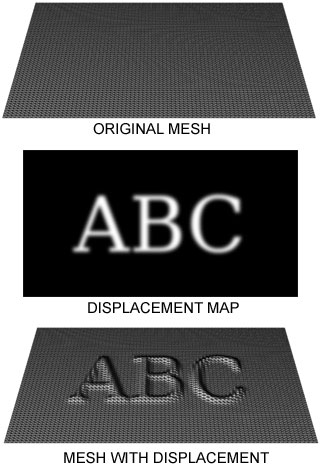
\includegraphics[width=110px]{pictures/displacement_mapping.jpg}
    \caption[Beispiel f"ur Displacement-Mapping]{Beispiel f"ur Displacement-Mapping \cite{displacement_mapping_pic}}
    \label{fig:displacement}
\end{figure}
dabei werden Texturen dazu verwendet, die Objektoberfl"ache zu alternieren.
Das hei\ss t, es werden nicht nur die Normalen, wie beim
Bump-Mapping ver"andert, um eine gew"unschte Erscheinung der Oberfl"ache zu
simulieren \cite{bump_mapping}, sondern es wird die tats"achliche
Objektgeometrie modifiziert.
Dies geschieht, indem die Vertices eines Objekts anhand der Werte einer
Displacement-Map entlang ihrer Normalen (senkrecht zur Oberfl"ache) verschoben
und die umliegenden Normalen entsprechend angepasst werden.\\
In Abbildung \ref{fig:displacement} ist ein
Beispiel f"ur eine solche
Displacement-Map und die Auswirkung auf eine Oberfl"ache (Mesh) gegeben.
Die Displacement-Map enth"alt dabei Farbwerte von schwarz (keine Ver"anderung)
bis wei\ss\ (maximale Verschiebung des Vertex in Richtung der Normalen).
Im dritten Bild ist die ver"anderte Silhouette der Oberfl"ache gut zu erkennen.
Da bei dieser Vertexverschiebung auch die Normalen neu berechnet werden,
sieht das Displacement-Mapping dem Bump-Mapping oftmals sehr "ahnlich, mit dem
entscheidenen Unterschied, dass die Struktur, die durch das Displacement-Mapping
erzeugt wird, im Umriss des Objekts sichtbar ist.


\section{Punkt-in-Polygon-Algorithmus}
\label{sec:pip_theo}
Der Punkt-in-Polygon-Algorithmus ist ein Verfahren um festzustellen, ob ein
gegebener Punkt in einer Ebene innerhalb oder au\ss erhalb der Grenzen
eines Polygons liegt. Diese Methode findet vorwiegend Anwendung bei der
Verarbeitung
Verarbeiten geometrischer Daten wie zum Beispiel in der Computergrafik.\\
Bereits 1974 wurden zwei Ans"atze zur L"osung des Punkt-in-Polygon-Problems
f"ur nicht-konvexe Polygone
(Ray-Casting und Winkelsummation) vorgestellt \cite[S. 13f.]{point_in_polygon}.
Sutherland verwendet den im Artikel vorgestellten Algorithmus um festzustellen
welche Oberfl"achen einer Szene n"aher am Betrachter liegen und welche
durch andere verdeckt werden.
\\
Im Folgenden wird n"aher auf das Konzept des Ray-Castings eingegangen, welches
in Abbildung \ref{fig:pip} illustriert wird.
\begin{figure}[htbp]
    \centering
    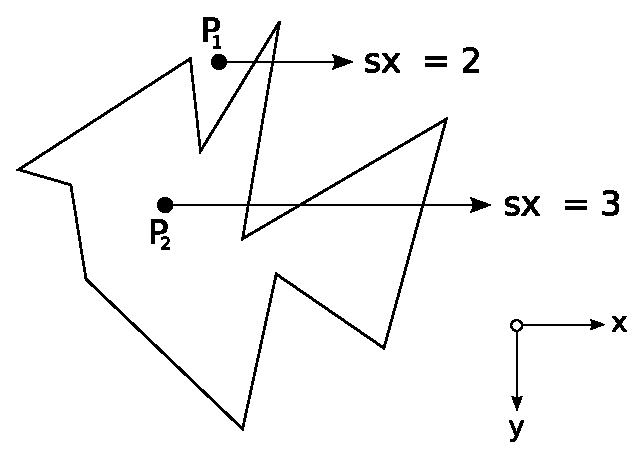
\includegraphics[width=200px]{pictures/punkt_in_polygon.eps}
    \caption{Punkt in Polygon Algorithmus}
    \label{fig:pip}
\end{figure}
Punkte werden getestet, indem man einen imagin"aren ''Strahl'' in eine
beliebige Richtung schickt und die Schnittpunkte mit den Kanten des Polygons
z"ahlt.
Ist die Anzahl der Schnittpunkte gerade, so liegt der Punkt
au\ss erhalb, ist sie ungerade, so liegt der Punkt innerhalb des Polygons.\\
Um konsistente Ergebnisse zu erhalten falls ein oder mehrere Polygon-Vertices
genau auf dem Test-Strahl liegen, ist es notwendig die Sonderf"alle zu
betrachten, die in Abbildung \ref{fig:sonderfaelle} dargestellt sind.
\begin{figure}[htbp]
    \centering
    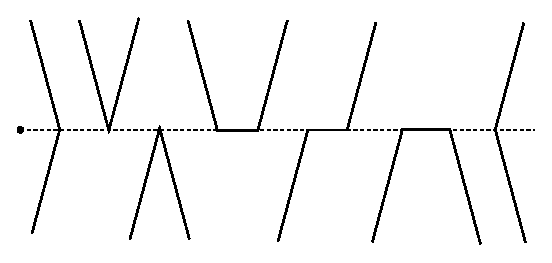
\includegraphics[width=250px]{pictures/sonderfaelle.eps}
    \caption{Sonderf"alle des Punkt in Polygon Algorithmus}
    \label{fig:sonderfaelle}
\end{figure}
Die Umgehung dieses Problems liegt in der Annahme, dass der Polygon-Vertex
infinitesimal "uber dem Test-Strahl liegt. Durch dieses Vorgehen wird
zus"atzlich festgelegt, zu welchem Polygon ein Pixel geh"ort, sollten
zwei Polygone einen oder mehrere Vertices gemeinsam haben
\cite[S. 51ff.]{skript_cg}.

\section{Marching-Cubes-Algorithmus}
\label{sec:mc_theo}
%Der MC geht auf Lorensen und Cline zur"uck...
\subsection{Bedeutung}
Der Marching-Cubes-Algorithmus wurde im Jahr 1987 im Auftrag der General
Electric Company von Lorensen und Cline entwickelt, um ein effizienteres
Verfahren zur Visualisierung medizinischer Messdaten bereitzustellen
\cite{marching_cubes}.
Bis zum damaligen Zeitpunkt wurde meist auf 2-dimensionale Bilddaten
von bildgebenden
Verfahren wie zum Beispiel der Computertomografie (CT) oder der
Magnetresonanztomografie (MRT) zur"uckgegriffen.
Da das Analysieren und Interpretieren dieser 2-dimensionalen Bilder
(Scheiben oder Schichten) besonderer Schulung und Erfahrung bedarf, bietet der
Marching-Cubes-Algorithmus
eine aussagekr"aftige, 3-dimensionale Repr"asentation der
evaluierten Messdaten zur
Unterst"utzung von Medizinern in den unterschiedlichsten Bereichen.\\
Die vom CT bzw. MRT erzeugten Volumendaten liegen in Form von Voxel-Datenmengen
vor. Das hei\ss t, dass in regelm"a\ss igen Abst"anden die Dichte des Materials
ermittelt und gespeichert wird, wodurch ein gleichm"a\ss iges 3-dimensionales
Datengitter generiert wird. Die Nachteile eines solchen Modells sind der enorme
Speicherbedarf und die langsame Visualisierung im Vergleich zu einfachen
Drahtgittermodellen.\\
Der Marching-Cubes-Algorithmus erm"oglicht nun, die
Voxel-Datenmengen durch ein polygonales Oberfl"achenmodell anzun"ahren und somit
effizient zu visualisieren.


\subsection{Funktionsweise}
Der Marching Cubes Algorithmus verfolgt einen Divide-and-Conquer-Ansatz.
Um die gegebenen Volumen-Daten zu Triangulisieren betrachtet man zun"achst zwei
benachbarte bzw. direkt "ubereinanderliegende Schichten oder Ebenen. In einem
n"achsten Schritt werden vier benachbarte Voxel auf der unteren Ebene
\texttt{z} so
miteinander verbunden, dass sie ein Quadrat ergeben. Danach werden diese mit
den genau dar"uberliegenden Voxeln der Ebene \texttt{z+1} zu einem imagin"aren
W"urfel erg"anzt (siehe Abbildung \ref{fig:mc}).
\begin{figure}[htbp]
    \centering
    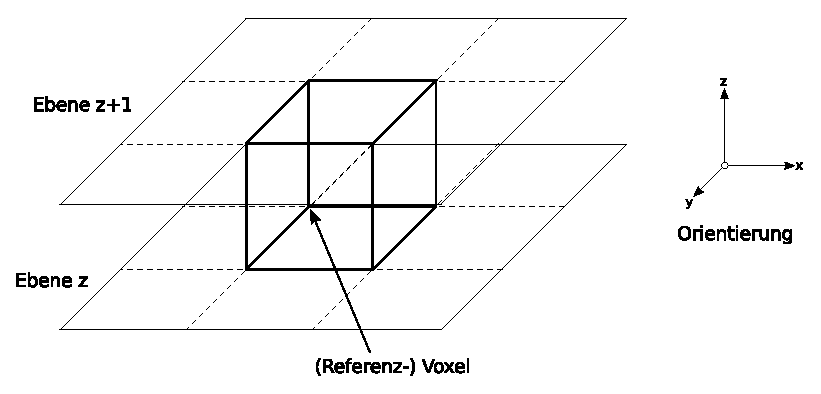
\includegraphics[width=300px]{pictures/marching_cube.eps}
    \caption{Marching-Cube}
    \label{fig:mc}
\end{figure}
Dabei gibt es meist einen Referenzvoxel, von dem aus die restlichen
Kubusecken mit Hilfe eines Offsets bestimmt werden.\\
Damit anschlie\ss end eine Oberfl"ache generiert werden kann, wird f"ur
jeden Eckpunkt
gepr"uft, ob dieser innerhalb oder au\ss erhalb des betrachteten Objektes liegt,
was anhand der Dichtewerte bestimmt werden kann.
Liegen alle Eckpunkte innerhalb oder au\ss erhalb, so muss dieser W"urfel nicht
weiter untersucht werden und es wird zum N"achsten ''marschiert''.
Liegt hingegen ein Schnittpunkt des Kubus mit der Objektoberfl"ache vor, so
teilt diese den Marching-Cube unweigerlich in Innen- und Au\ss enbereiche.\\
Da der W"urfel acht Eckpunkte besitzt, gibt es genau $2^8 = 256$ M"oglichkeiten,
den Kubus zu zerteilen.
Aus Symmetriegr"unden k"onnen diese 256 F"alle auf die in Abbildung
\ref{fig:mc_possibilities} dargestellten 15 reduziert
werden.
\begin{figure}[htbp]
    \centering
    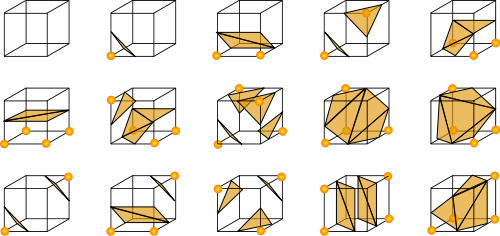
\includegraphics[width=350px]{pictures/marchingCubes.png}
    \caption[Schnittm"oglichkeiten eines W"urfels]
        {Schnittm"oglichkeiten eines W"urfels \cite{mc_possibilities}}
    \label{fig:mc_possibilities}
\end{figure}
Sind schlie\ss lich die Zust"ande aller beteiligten Voxel bestimmt, so wird in
einer Tabelle, der sogenannten
\texttt{TriangleLookupTable} nachgesehen, welche Dreiecke in dem vorliegenden
Fall gezeichnet werden m"ussen. Genauer gesagt werden die W"urfelkanten,
die von der Oberfl"ache geschnitten werden und
zus"atzlich die Eckpunkte der zu zeichnenden Dreiecke bestimmt.
In Kapitel \ref{sec:mc_algo} wird dieses Verfahren und die \texttt{TriangleLookupTable}
genauer erl"autert.\\
Wahlweise k"onnen f"ur eine bessere Ann"aherung an das Ursprungsobjekt die
Oberfl"achenpunkte entsprechend interpoliert werden. Ansonsten wird f"ur die
Berechnung der Dreiecke immer von der Mitte einer W"urfelkante ausgegangen.
Zur besseren Darstellung (Beleuchtung) lassen sich daraufhin die
Einheitsnormalen berechnen.\\
Ein Beispiel f"ur die Visualisierung eines aus 150 Schichten bestehenden
MRT-Modells soll die Abbildung \ref{fig:mc_head} geben, in der die
Ann"aherung an einen Kopf deutlich zu erkennen ist.
\begin{figure}[htbp]
    \centering
    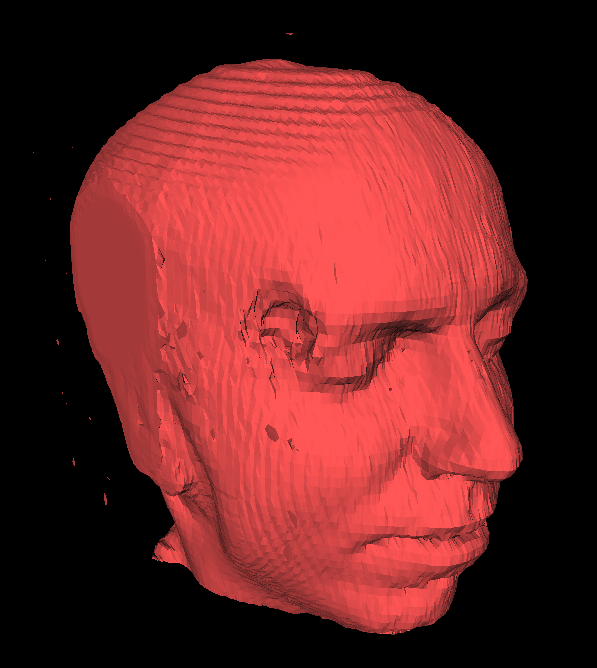
\includegraphics[width=180px]{pictures/marching_cubes_head.png}
    \caption[Marching-Cubes - Polygonmodell eines Kopfes]
        {Marching-Cubes - Polygonmodell eines Kopfes \cite{mc_head}}
    \label{fig:mc_head}
\end{figure}




%%%%%%%  UMSETZUNG  %%%%%%%%

\chapter{Umsetzung}

%%%% TODO evtl. umschreiben, oder weglassen
%Dieses Kapitel besch"aftigt sich mit der Umsetzung und Implementierung der
%vorher genannten Konzepte. Nach einer Darstellung verschiedener
%L"osungsans"atze wird genauer auf den gew"ahlten Ansatz eingegangen.
%Besonders herausgestellt werden der Punkt in Objekt Algorithmus sowie der
%Marching Cubes Algorithmus, die den Kern dieser Arbeit darstellen.


\section{Ans"atze}
Dieses Kapitel befasst sich mit m"oglichen L"osungsans"atzen zur Erstellung
einer Schneedecke und stellt drei verschiedene Ans"atze dar, von denen der
Letztgenannte umgesetzt werden soll.


\subsection{Snow-Map}
\subsubsection{Interpretation als Lightmap}
Ein erster, naiver Ansatz, eine Schneedecke zu modellieren ist es, eine Textur
zu erstellen, die die Aufgabe hat, die Menge an gefallenem Schnee an jeder
Stelle der Szene zu speichern. Diese Textur wird im Folgenden als Snow-Map
bezeichnet.
Die Snow-Map k"onnte anschlie\ss end "ahnlich wie eine Lightmap
interpretiert werden. Das hei\ss t, dass in die urspr"ungliche Farbe der
Objekttextur entsprechend der Menge an Schnee wei\ss\ hineingemischt wird um
die Farbe aufzuhellen. Das Prinzip
einer Lightmap ist in Abbildung (\ref{fig:lightmap}) verdeutlicht.
\begin{figure}[htbp]
    \centering
    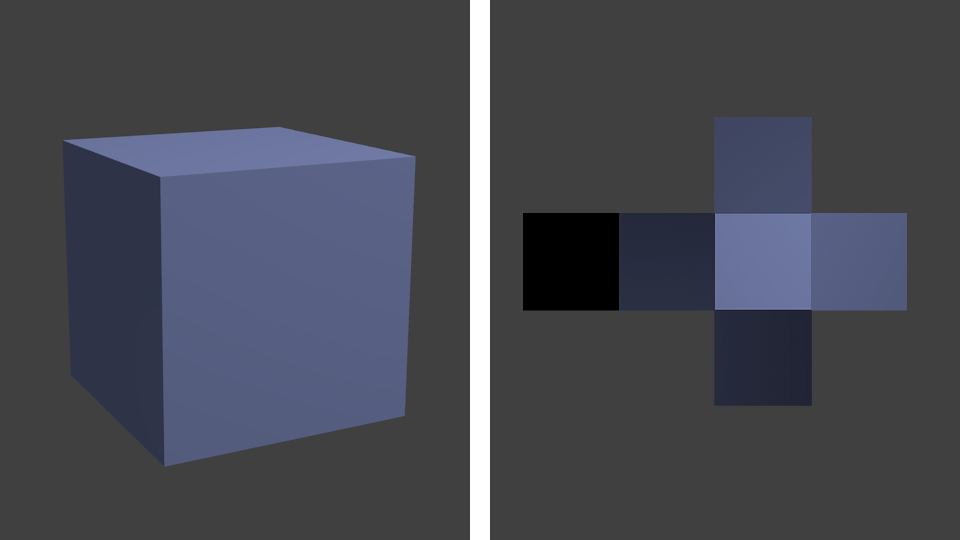
\includegraphics[width=350px]{pictures/lightmap.png}
    \caption{Lightmap auf einer Wand}
    \label{fig:lightmap}
\end{figure}
Die Abbildung zeigt die Auswirkung einer Lightmap in Form eines Spotlights
auf eine Mauer-Textur.
Ebenso w"urde sich die Snow-Map bei der Simulation von
Schnee verhalten.
Die dabei
entstehenden Probleme liegen auf der Hand. Es k"onnen lediglich hellere Stellen
oder Fl"achen auf der bereits vorhandenen Oberfl"ache entstehen. L"auft die
Simulation lange genug, bzw. f"allt gen"ugend Schnee, so ist nach gewisser Zeit
die gesamte Oberfl"ache der Szene wei\ss\ und eine Unterscheidung zwischen
viel und wenig Schnee ist nicht mehr m"oglich. Die Nutzung einer einfachen
Textur bedeutet letztlich, dass keine richtige Schneedecke vorhanden ist,
wodurch wiederum keine Schneeh"aufungen oder -ansammlungen deutlich gemacht
werden k"onnen.
Dieser Ansatz f"uhrt folglich zu keinem zufriedenstellenden Ergebnis.


\subsubsection{Interpretation als Light- und Displacement-Map}
Zur Verbesserung des Ergebnisses, das allein mit der Lightmap erzeugt werden
kann, w"are es denkbar, die Snow-Map als eine Kombination aus Light- und
Displacement-Map zu interpretieren. Dabei arbeitet die Lightmap
wie im vorherigen Abschnitt beschrieben,die Funktionsweise der
Displacement-Map ist Kapitel \ref{sec:displacement_mapping} zu entnehmen.\\
Zus"atzlich zu der dort gegebenen Beschreibung w"urde man eine Schneegeometrie
definieren, die initial mit der Szenengeometrie "ubereinstimmt, und die Werte in
der Snow-Map als Transparenzfaktor betrachten. Damit ist gemeint, dass, je
dunkler der Farbwert in der Snow-Map ist, desto transparenter erscheint die
Schneegeometrie an dieser Stelle, so dass man die Szene darunter noch erkennen
kann. Umgekehrt ist die Schneegeometrie undurchsichtiger, je heller der Wert
der Snow-Map ist.
Hierbei ist es wichtig zu bedenken, dass die Schneegeometrie von Anfang an
wei\ss\ ist und nur die Transparenz die Menge an Schnee wiederspiegelt.
\begin{figure}[htbp]
    \centering
    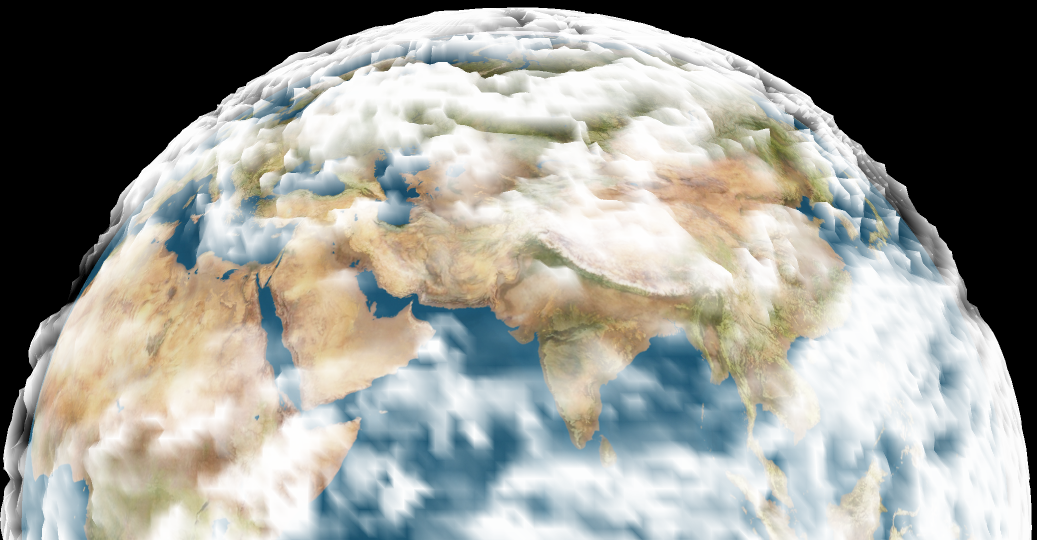
\includegraphics[width=350px]{pictures/clouds.png}
    \caption[Beispiel f"ur transparentes Displacement-Mapping]
        {Beispiel f"ur transparentes Displacement-Mapping \cite{wenke}}
    \label{fig:clouds}
\end{figure}
Somit lie\ss en sich Erhebungen und Schneeh"aufungen darstellen, die zudem
passend eingef"arbt w"aren. Jedoch wird man bei dieser Vorgehensweise ebenfalls
mit gewissen Problemen konfrontiert.
Zwar ist das Ergebnis bei einem steilen Betrachtungswinkel durchaus
zufriedenstellend, jedoch kann es bei der Visualisierung
passieren, dass aufgrund der Transparenz bei einem flachen Betrachtungswinkel
lediglich schwebende
Pyramiden- bzw. Kegelspitzen zu sehen sind (vgl. Rand der Erdkugel in
Abbildung \ref{fig:clouds}).
Des Weiteren k"onnen unerw"unschte "Uberschneidungen in der N"ahe von
Objektecken auftreten.
\begin{figure}[htbp]
    \centering
    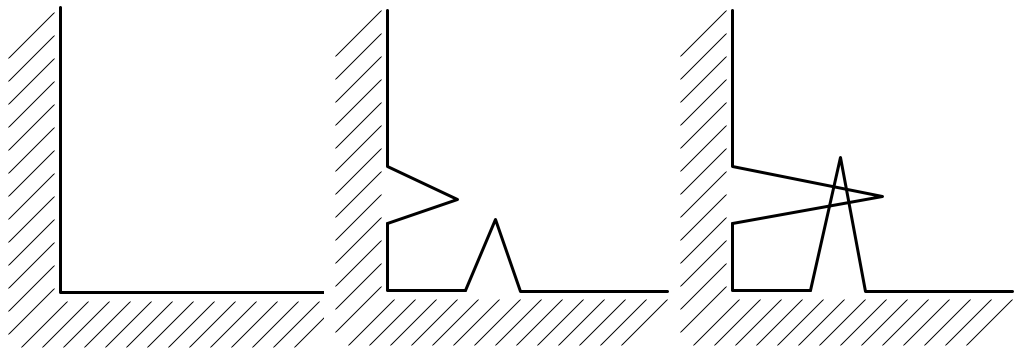
\includegraphics[width=300px]{pictures/ecke.png}
    \caption{"Uberschneidung beim Displacement-Mapping}
    \label{fig:ecke}
\end{figure}
Ein m"ogliches Problem ist in Abbildung \ref{fig:ecke} aufgezeigt. Aufgrund
der sich ver"andernden Schneegeometrie und eventuell wachsenden Schneemengen
k"onnte es zu "Uberschneidungen der Schneedecke mit sich selbst kommen (siehe Bild 3). Da allerdings weder schwebende Kegelspitzen
sichtbar sein, noch seltsame Effekte beim Rendern durch
"Uberschneidungen auftreten sollen,
kann auch dieser Ansatz kein befriedigendes Ergebnis liefern.


\subsection{Voxelrepr"asentation}
\label{sec:voxel}
Die L"osung des Problems der bisher fehlenden Schneedecke, beziehungsweise
der sich selbst schneidenden Displacement-Oberfl"ache kann mit Hilfe der
Repr"asentation durch Voxel realisiert werden.
\begin{figure}
    \centering
    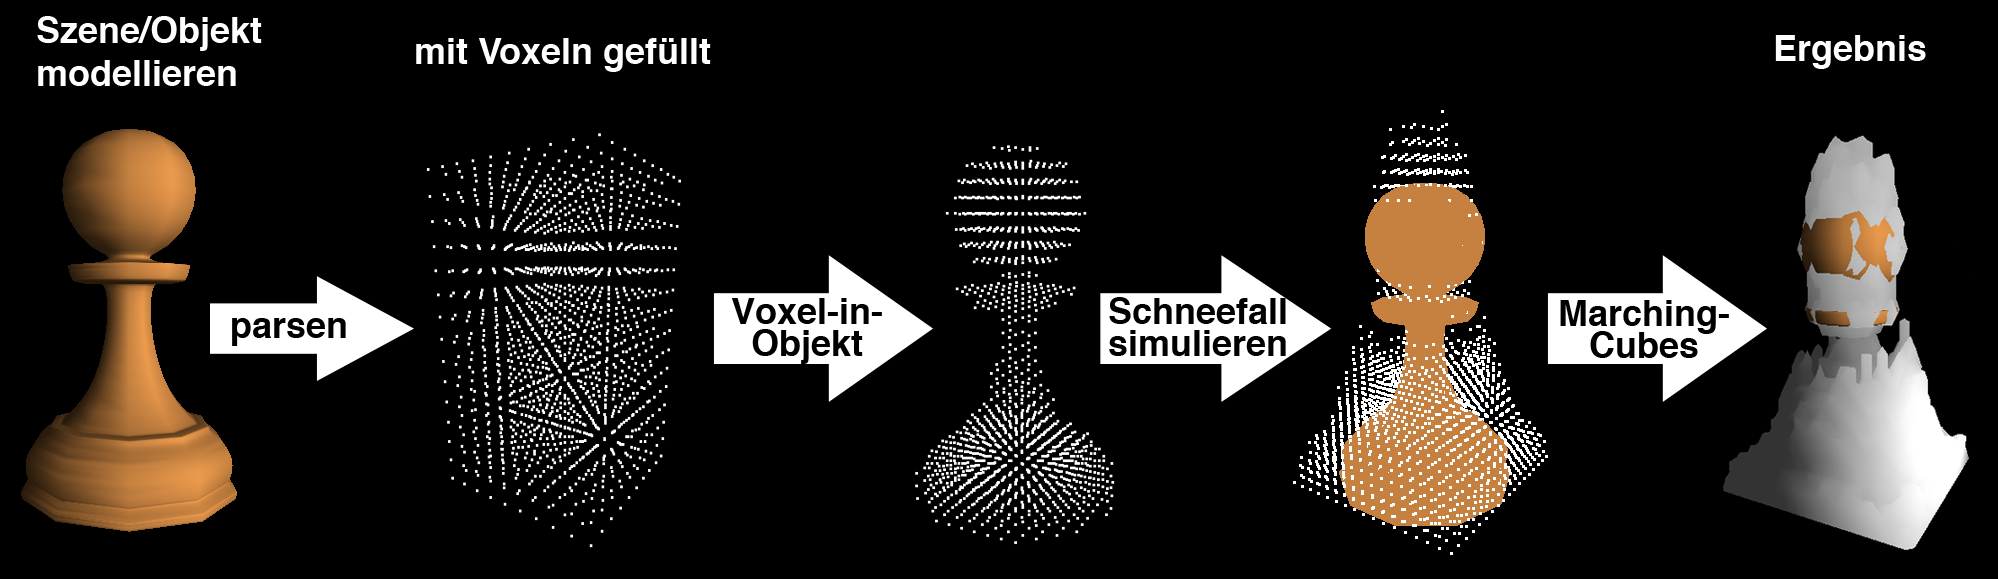
\includegraphics[width=450px]{pictures/snow_pipeline.png}
    \caption{Snow-Pipeline}
    \label{fig:snow_pipeline}
\end{figure}
Dabei wird basierend auf Voxeln eine
\glqq richtige\grqq\ Schneedecke erzeugt, die auf bzw. "uber der Szenenoberfl"ache
liegt. Dies wird erreicht, indem der gesamte Raum, den die Szene einnimmt,
mit Voxeln gef"ullt wird, sodass die Schneedecke sp"ater "uberall wachsen
kann. Darauffolgend wird f"ur jeden Voxel gepr"uft, ob er innerhalb oder
au\ss erhalb eines Objektes liegt, um im Anschlu\ss\ mit Hilfe des
sogenannten Marching-Cubes-Algorithmus' (siehe Kapitel \ref{sec:mc_algo})
eine Schneedecke zu erzeugen (siehe Kapitel \ref{sec:snow_surface}).
Demnach ist keine "Uberschneidung der Displacement-Oberfl"ache
in den Ecken mehr m"oglich, da die Voxel in einem regelm"a\ss igen
Gitter gesetzt werden und jeder Voxel nur einmal existiert.
\begin{figure}[htbp]
    \centering
    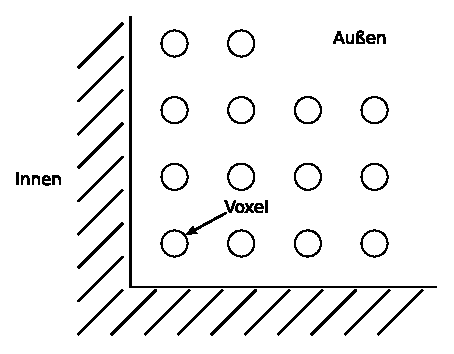
\includegraphics[width=180px]{pictures/voxel.eps}
    \caption{Voxel in Objektecken}
    \label{fig:voxel}
\end{figure}
Die Abbildung \ref{fig:voxel} verdeutlicht das gleichm"a\ss ige Voxelgrid
sowie die L"osung des "Uberschneidungsproblems.
W"achst die Schneedecke beispielsweise von
unten und von links an, so trifft die Schneeoberfl"ache irgendwann auf
denselben Voxel und dieser merkt sich, dass er nun Schnee beinhaltet.
Die Schneedecke erweitert sich anschlie\ss end von beiden Seiten bis zu diesem
Punkt. Folglich kann es keine
ungewollten "Uberschneidungen geben. Die Bereiche \glqq Innen\grqq\ und
\glqq Au\ss en\grqq\
stehen in der Zeichnung f"ur Gebiete innerhalb bzw. au\ss erhalb eines
Objekts.
\\
Im Folgenden wird erl"autert, was ein Voxel genau ist, welche
Eigenschaften er hat und welche Bedeutung diese f"ur den weiteren Verlauf
der Arbeit haben.

\subsubsection{Voxel}
Wie zuvor bereits angedeutet, sind Voxel im Grunde Punkte im Raum, die gewisse
Eigenschaften besitzen.
Ein Voxel wird folglich durch eine \texttt{x}-, \texttt{y}- und
\texttt{z}-Koordinate zur eindeutigen Festlegung der Position definiert.
Des Weiteren wird gespeichert, ob sich ein Voxel inner- oder au\ss erhalb
eines Objekts befindet, was mit Hilfe des dreidimensionalen
Punkt-in-Polygon-Algorithmus'
ermittelt wird. Zudem wird vorgehalten, ob ein Voxel Schnee
beinhaltet. Ist dies der Fall, so wird in einer weiteren Variablen ein
gewisser \texttt{density}-Wert festgehalten, der aussagt, wie viel
Schnee der Voxel enth"alt.\\
Als letzte wichtige Information merkt sich jeder Voxel seine bis zu sechs
direkten Nachbarn. Die zugrunde liegende Nachbarschaftsbeziehung ist in
Abbildung \ref{fig:voxel_neighborhood} dargestellt.
\begin{figure}[htbp]
    \centering
    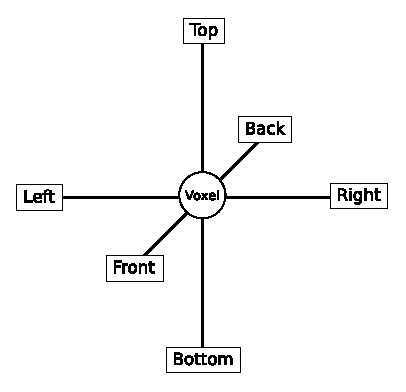
\includegraphics[width=180px]{pictures/neighborhood.eps}
    \caption{Voxelnachbarschaft}
    \label{fig:voxel_neighborhood}
\end{figure}
Ein Voxel in der Szenenmitte hat somit stets 6 Nachbarn, Randvoxel haben 5,
Voxel auf einer Szenenkante 4 und die Voxel in den vier Eckpunkten haben
lediglich 3 direkte Nachbarn.


\subsubsection{1. Ansatz: rechteckige/rasterangepasste Objekte}
Ein erster, einfacher Ansatz zur Repr"asentation einer Schneedecke durch Voxel
ist in Abbildung \ref{fig:voxel_grid_rect}
dargestellt. Die Kreise repr"asentieren Voxel, wobei diese rot eingef"arbt
sind, wenn sie in einem Objekt liegen.
Zur besseren "Ubersicht sind die Abbildungen in diesem Abschnitt
zweidimensional.
\begin{figure}[htbp]
    \centering
    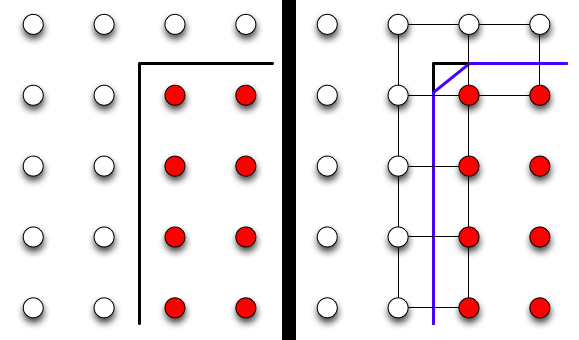
\includegraphics[width=200px]{pictures/voxel_grid_rect.png}
    \caption{Beispiel eines rechteckigen Objektes im Voxelgrid}
    \label{fig:voxel_grid_rect}
\end{figure}
Gegeben ist ein rechteckiges Objekt, dessen Kanten exakt
zwischen den Voxeln liegen (linkes Bild). In diesem Fall liefert der
Marching-Cubes-Algorithmus ein sehr gutes Ergebnis, da er als Grundlage
f"ur die Schnittpunktberechnung im Standardfall die Kantenmitte zugrunde legt.
Involvierte bzw. geschnittene W"urfel sind als solche hervorgehoben.
Die resultierende, initial erzeugte Oberfl"ache ist im rechten Bild durch die
blaue Linie gekennzeichnet und stimmt fast exakt mit der Oberfl"ache des
Objekts "uberein.


\subsubsection{2. Ansatz: beliebige Objekte}
Der zweite Ansatz verfolgt nun das Ziel, das Ergebnis des ersten Ansatzes f"ur
beliebige Objekte zu erzeugen.
Um folglich eine Oberfl"ache wie im linken Bild der Abbildung
\ref{fig:voxel_grid_random}
m"oglichst exakt nachzubilden, m"ussen die Schnittpunkte zwischen den
Kuben und der Objektoberfl"ache entsprechend genau berechnet bzw. interpoliert
werden.
\begin{figure}[htbp]
    \centering
    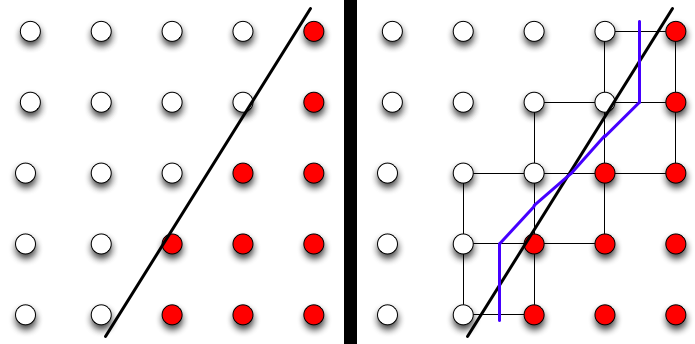
\includegraphics[width=200px]{pictures/voxel_grid_random.png}
    \caption{Beispiel eines beliebigen Objektes im Voxelgrid}
    \label{fig:voxel_grid_random}
\end{figure}
Setzt man bei einer solchen beliebigen Oberfl"ache die Schnittpunkte in die Kantenmitte, so erh"alt man eine initial angen"aherte L"osung, die durch
die blaue Linie im rechten Bild dargestellt wird.
Es ist deutlich zu sehen, dass die Oberfl"ache teilweise "uber und teilweise
unter der tats"achlichen Objektoberfl"ache liegt. Dies kann dazu f"uhren,
dass die Schneedecke leicht "uber dem Objekt schwebt.\\

Aufgrund der h"oheren Komplexit"at des zweiten Ansatzes wird in der
vorliegenden Arbeit der erste Ansatz verfolgt und umgesetzt. Dies hat
zur Folge, dass die durch das Programm erzeugten Ergebnisse f"ur Objekte
optimiert sind, deren Kanten mit dem Voxelgitter "ubereinstimmen, also
vorwiegend rechteckig sind. Nat"urlich werden auch Ergebnisse f"ur beliebige
Objekte geliefert, diese sind allerdings aus den oben genannten Gr"unden
unpr"aziser. Nat"urlich erh"oht sich die Qualit"at des Ergebnisses mit
steigender Anzahl von Voxeln, welche ab einer bestimmten Menge und
Szenengr"o\ss e jedoch unpraktikabel wird. Zudem spielt dies nur bei der
ersten Anwendung des Marching-Cubes-Algorithmus' eine Rolle, denn sobald die
Schneedecke anw"achst, soll diese "uber dem Objekt liegen. In Kapitel
\ref{sec:snow_surface} wird dieses Problem erneut aufgegriffen und
anhand von Applikationsgrafiken illustriert.


\section{Szene auslesen}
Um nun eine Schneedecke simulieren zu k"onnen, muss die vorliegende Szene
zun"achst ausgelesen werden.
Das im Zusammenhang mit dieser Arbeit entstandene Programm kann beliebige Szenen
im Wavefront-Format einlesen.
%TODO mehr Informationen ueber das Format, woher kommt es, Verbreitung, etc.
%Hierbei ist es wichtig, dass die Szene in dem sogenannten
%Wavefront-Dateiformat (Dateiendung: *.obj) vorliegt.
Es folgt eine
kurze Erkl"arung dieses
Dateiformats sowie die Beschreibung und Funktionsweise des Parsers.

\subsection{Wavefront-Dateiformat}
Eine Wavefront-Datei enth"alt alle f"ur die Szene relevanten Informationen,
wie Vertices, Normalen, Faces, Texturkoordinaten oder benutzte
Oberfl"achenmaterialien.
In dem folgenden Dateiausschnitt sind die f"ur diese Applikation erforderlichen
Daten beispielhaft aufgef"uhrt.
\inputminted[]{ruby}{code/cube.obj}
Die ersten beiden Zeilen k"onnen ignoriert werden, da es Kommentare sind,
deren Inhalt hier irrelevant ist.
Es sind lediglich jene Zeilen von Bedeutung, die mit \glqq\texttt{v}\grqq\,
\glqq \texttt{vn}\grqq\ oder \glqq\texttt{f}\grqq\ beginnen.\\
Das Pr"afix \glqq\texttt{v}\grqq\ leitet einen Vertex ein, gefolgt von den
zugeh"origen
\texttt{x}-, \texttt{y}- und \texttt{z}-Koordinaten, welche jeweils durch ein
Leerzeichen getrennt sind.
Analog dazu sind die Vertexnormalen aufgelistet, die durch das Pr"afix
\glqq\texttt{vn}\grqq\ eingeleitet werden, mit dem Unterschied, dass die
Koordinaten
keine Position, sondern eine Richtung angeben.\\
Sowohl f"ur die Vertices als auch f"ur die Normalen gilt, dass sie nur einmal
aufgelistet werden. Sollten beispielsweise an der selben Stelle mehrere
Vertices liegen, so wird dieser eine Vertex nicht mehrfach aufgef"uhrt, sondern
mehrfach verwendet (z.B. wenn mehrere Faces den selben Vertex als
Eckpunkt verwenden). Dies geschieht mit Hilfe einer impliziten Indizierung.
Jeder Vertex und jede Normale hat einen eindeutigen Index, der durch ihre
jeweilige Position in der Liste gegeben ist.\\
Die implizite Indizierung der Datei sieht nun wie folgt aus:

\inputminted[]{ruby}{code/cube_index.obj}

Schlie\ss lich leitet das Pr"afix \glqq\texttt{f}\grqq\ ein Face ein.
Hinter jedem
\glqq\texttt{f}\grqq\ stehen drei durch Leerzeichen getrennte Strings
in dem Format
\glqq\texttt{<vertex\_index>//<normal\_index>}\grqq\.\\
Somit wird festgelegt, welche Vertices miteinander zu einem Face verbunden
werden m"ussen und welche Normale der jeweilige Vertex hat. Zum Beispiel:

\inputminted[]{ruby}{code/face.obj}

Dieses Face besteht folglich aus dem Vertex mit dem Index 5, dem Vertex
mit dem Index 8
und dem Vertex mit dem Index 7, welche in genau dieser Reihenfolge miteinander verbunden
werden. Alle drei Vertices haben hier die Normale mit dem
Index 2.


\subsection{Parser}
Mit dem oben beschriebenen Wissen "uber das vorliegende Dateiformat kann nun
ein entsprechender Parser zum Auslesen der Szene entwickelt werden. Dieser
liest die Werte ein und speichert sie zur weiteren Verarbeitung in mehreren
Arrays.\\
Dabei wird zun"achst die gesamte Datei durchgegangen um die Vorkommen der
\glqq\texttt{v}\grqq\, \glqq\texttt{vn}\grqq\ und \glqq\texttt{f}\grqq\ zu z"ahlen und entsprechend
gro\ss e Arrays anzulegen. Diese Arrays sind:

\begin{itemize}
    \item{\textbf{vertexArray}}: Enth"alt die Vertex-Koordinaten, die
        hintereinander in das Array eingetragen werden.
    \item{\textbf{normalArray}}: Enth"alt die (Richtungs-) Koordinaten der
        Normalen, die ebenfalls hintereinander in dem Array stehen.
    \item{\textbf{faceArray}}: Enth"alt die Indizes der Vertices die zu einem
        Face verbunden werden. Ein Face besteht dabei immer aus drei Vertices.
    \item{\textbf{normalIndexArray}}: Enth"alt analog zum \texttt{faceArray}
        die Indizes der Normalen.
\end{itemize}

Nachdem die Arrays erstellt wurden, wird die Datei mit Hilfe der folgenden
\texttt{while}-Schleife durchgegangen um die Arrays zu f"ullen.

\inputminted[linenos=true]{java}{code/Parser.java}

Hierbei werden jeweils die ersten zwei Zeichen jeder Zeile mit den oben
genannten Pr"afixen (hier rep"asentiert durch Konstanten) verglichen, wodurch
festgestellt wird, ob es sich um
einen Vertex, eine Normale oder ein Face handelt. Je nach "Ubereinstimmung
wird die entsprechende Methode aufgerufen, welche die Werte der Zeile
in das korrekte Array eintr"agt. Dabei ist zu erw"ahnen,
dass die Methode \texttt{addFaces(String line)} beiden Index-Arrays
(\texttt{faceArray} und \texttt{normalIndexArray}) ihre Werte zuweist, da dort
immer zwei Informationen in einer Zeile stehen.

%%%%%%%% Hier evtl. noch Zugriff auf Daten erkl"aren

\section{Szene mit Voxeln f"ullen}
\label{sec:voxel_fill}

Nachdem die Szene nun ausgelesen werden kann und die Arrays mit den ben"otigten
Daten zur Verf"ugung stehen, soll die Szene mit Voxeln gef"ullt werden.
%TODO oberen Abschnitt umschreiben (Erzaehlstil)
\\
Um ein regelm"a\ss iges Voxelgitter zu erstellen, muss als erstes
die r"aumliche Ausdehnung der Voxel
bestimmt werden, das hei\ss t, die Gr"o\ss e der Szene ist
zu ermitteln. Mit Hilfe des Vertex-Arrays l"asst sich nun der gr"o\ss te bzw.
kleinste in der Szene enthaltene Wert auf jeder der drei Achsen herausfinden.
Daraus lassen sich drei Kantenl"angen berechnen, aus denen wiederum ein
Quader ermittelt werden kann, der die Szene enth"alt und mit Voxeln
aufgef"ullt wird.
%TODO weglassen
%Beispielhaft sei hier die Methode zur Berechnung des gr"o\ss ten
%\texttt{x}-Wertes dargestellt.
%\inputminted[linenos=true]{java}{code/CalculateMaxX.java}
%Die Methode bekommt das gesamte Vertex-Array "ubergeben und geht alle Vertices
%durch, wobei lediglich die \texttt{x}-Koordinate betrachtet wird (Zeile 7).
%Es wird sich der bisher gr"o\ss te gefundene \texttt{x}-Wert gemerkt und
%bei Bedarf aktualisiert und am Ende zur"uckgegeben.\\
%Die Berechnung der f"unf weiteren Werte geschieht analog, mit dem Unterschied,
%dass die untersuchte Koordinate des Vertex wechselt.\\
Um den Quader mit Voxeln zu f"ullen wird die folgende Methode verwendet.

\inputminted[linenos=true]{java}{code/FillScene.java}

Man geht entlang jeder Koordinatenachse die zuvor berechnete Kantenl"ange
ab und setzt einen Voxel an den entsprechenden Koordinaten. Um alle drei
Dimensionen abzuarbeiten, wird dieses Vorgehen mit drei ineinander
geschachtelten \texttt{for}-Schleifen realisiert.
Die Konstante \texttt{STEPS} stellt eine Art Granularit"atsfaktor dar,
das hei\ss t, pro L"angeneinheit im Koordinatensystem werden \texttt{STEPS}
Voxel gesetzt.\\
%TODO evtl. die setVoxel()-Methode erkl"aren
Das Ergebnis ist in Abbildung \ref{fig:pawn_scene} zu sehen.
\begin{figure}[htbp]
    \centering
    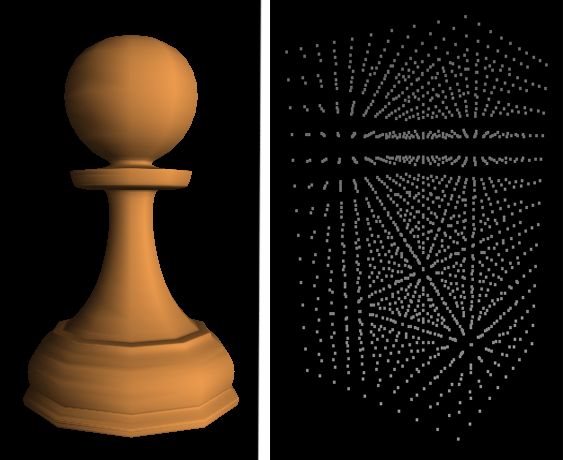
\includegraphics[width=200px]{pictures/pawn_scene.png}
    \caption{Voxelgitter}
    \label{fig:pawn_scene}
\end{figure}
Als Grundlage der Szene wurde beispielhaft ein Bauer eines Schachspiels
herangezogen (links im Bild). Die rechte Bildh"alfte stellt die ausgelesene
Szene dar, in der nur die gesetzten Voxel angezeigt werden.\\
Nachdem die Szene gef"ullt und alle ben"otigten Voxel erzeugt wurden, sind
im Anschluss die Nachbarschaftsbeziehungen f"ur jeden Voxel zu setzen.
Exemplarisch sei einmal die Bestimmung des rechten Nachbarvoxels aufgef"uhrt.

\inputminted[linenos=true]{java}{code/SetRightNeighbor.java}

Die Methode bekommt das gesamte Voxelgitter sowie die Distanz zwischen zwei
benachbarten Voxeln "ubergeben. Die Distanz h"angt von der zuvor bestimmten
Voxeldichte ab. Es wird f"ur jeden Voxel der Szene gepr"uft, ob dieser die
richtigen Bedingungen erf"ullt. Zun"achst wird der Abstand zwischen
dem aktuellen Voxel und dem untersuchten auf der \texttt{x}-Achse berechnet
(Zeile 5) und in \texttt{tmp} gespeichert. F"ur diesen Abstand muss nun gelten,
dass er der vorgegebenen Distanz entspricht und positiv ist, da der rechte
Nachbarvoxel auch rechts vom aktuellen Voxel liegen sollte. Weiterhin
ist zu beachten, dass der Nachbarvoxel auf derselben H"ohe
(gleiche \texttt{z}-Koordinate) sowie direkt neben (gleiche
\texttt{y}-Koordinate) dem Referenzvoxel liegen muss.\\
Wurde ein passender Kandidat gefunden, so wird sich dieser gemerkt und die
Methode kann verlassen werden, da es h"ochstens einen rechten Nachbarn geben
kann.
Die Bestimmung der f"unf restlichen Nachbarn erfolgt analog. Dieser Prozess
kann abh"angig von der Granularit"at eine gewisse Zeit beanspruchen,
da f"ur jeden Voxel das gesamte Voxelgrid linear durchsucht
werden muss.


\section{Voxel-in-Objekt-Algorithmus}
\label{sec:voxel_in_object}
In diesem Abschnitt soll die Funktionsweise des 3-dimensionalen Punkt in
Polygon Algorithmus erl"autert werden. Mit den daraus gewonnenen Informationen
l"asst sich
sp"ater bestimmen, an welchen Stellen der Szene Schnee fallen kann und an
welchen nicht.
%TODO groben Ueberblick schaffen, WARUM wird das ueberhaupt gemacht?


\subsection{Aktive Faces berechnen}
Es sollen nicht immer alle in der Szene
enthaltenen Faces auf Schnittpunkte mit dem aus dem
Punkt-in-Polygon-Algorithmus bekannten
imagin"aren \glqq\ Strahl\grqq\ gepr"uft werden, sondern lediglich die
f"ur die jeweilige Ebene relevanten.\\ %%%%% TODO Umschreiben!!!!
Da der Algorithmus die Szene ebenenweise durchgeht, m"ussen die Faces, die die
aktuelle Ebene schneiden, nur ein Mal pro Ebene ermittelt werden. Das bedeutet,
dass alle Voxel in der aktuellen \texttt{x}-\texttt{y}-Ebene dieselbe
\texttt{z}-Koordinate
besitzen und nur mit den gerade aktiven Faces gepr"uft werden m"ussen.
\inputminted[linenos=true]{java}{code/ActiveFaces.java}
Welches Face die betrachtete Ebene schneidet, bestimmt die
\texttt{z}-Koordinate der drei Face-Vertices. Sind alle
\texttt{z}-Werte kleiner oder gr"o\ss er als der \texttt{z}-Wert der Ebene,
so gibt es offensichtlich keine Schnittkante. Sobald eine
\texttt{z}-Koordinate gr"o\ss er und eine andere kleiner ist als die der Ebene,
muss es einen Schnitt geben und das Face wird zu den aktiven Faces
hinzugef"ugt. Diese Abfrage findet in dem \texttt{if}-Statement im oberen
Code-Ausschnitt statt (Zeilen 8-13).
\begin{figure}[htbp]
    \centering
    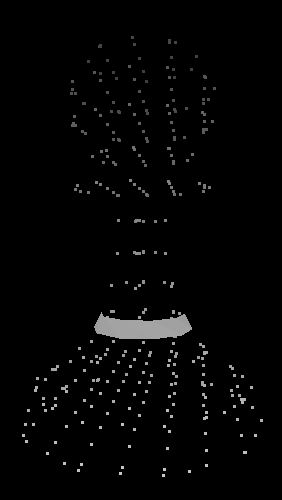
\includegraphics[width=120px]{pictures/active_faces.png}
    \caption{Aktive Faces}
    \label{fig:active_faces}
\end{figure}
In Abbildung \ref{fig:active_faces} sind die aktiven Faces f"ur eine Ebene
dargestellt. Zudem werden zur besseren "Ubersicht lediglich
die innenliegenden Voxel angezeigt.\\
In einem n"achsten Schritt m"ussen nun die genauen Schnittkanten der Faces mit
der entsprechenden Ebene berechnet werden.


\subsection{Schnittkanten der Faces mit der Ebene bestimmen}
\label{sec:schnittkanten}
Die Schnittkantenberechnung der aktiven Faces mit der aktuell betrachteten
Ebene ist entscheidend, um im Anschluss den zweidimensionalen
Punkt-in-Polygon-Algorithmus anwenden zu k"onnen.\\
Dazu werden zun"achst alle M"oglichkeiten, ein Face zu schneiden, betrachtet
(siehe Abbildung \ref{fig:faces_schnitte}).
\begin{figure}[htbp]
    \centering
    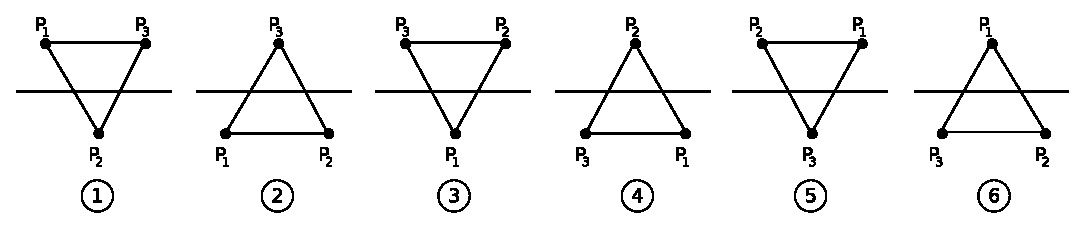
\includegraphics[width=400px]{pictures/faces_schnitte.eps}
    \caption{Schnittm"oglichkeiten: Ebene - Face}
    \label{fig:faces_schnitte}
\end{figure}
Es k"onnen sechs verschiedene F"alle unterschieden werden. F"ur die
Fallunterscheidung signifikant sind die
\texttt{z}-Koordinaten der drei Vertices jedes Faces. Es wird gepr"uft, welcher
Vertex oberhalb und welcher unterhalb der Ebene liegt. Aus Symmetriegr"unden
k"onnen bei der weiteren Berechnung die F"alle \texttt{1} und \texttt{4},
\texttt{2} und \texttt{5} sowie \texttt{3} und \texttt{6} zusammengefasst
werden, da jeweils die gleichen Seiten des Face-Dreiecks geschnitten werden.\\
Um die genaue
Schnittkante zwischen Face und Ebene zu berechnen, wird bestimmt,
welche beiden Seiten des Faces geschnitten werden. Aus den daraus
resultierenden Schnittpunkten l"asst sich anschlie\ss end die
Schnittkante zusammensetzen.\\
Das bedeutet, dass f"ur jedes Face zweimal ein Schnittpunkt zwischen einer
Geraden und der aktuellen Ebene durchgef"uhrt werden muss.
Umgesetzt wird dies mit Hilfe einfacher Vektorgeometrie. Zur besseren
Veranschaulichung ist Abbildung \ref{fig:sp_gerade_ebene} gegeben.
\begin{figure}[htbp]
    \centering
    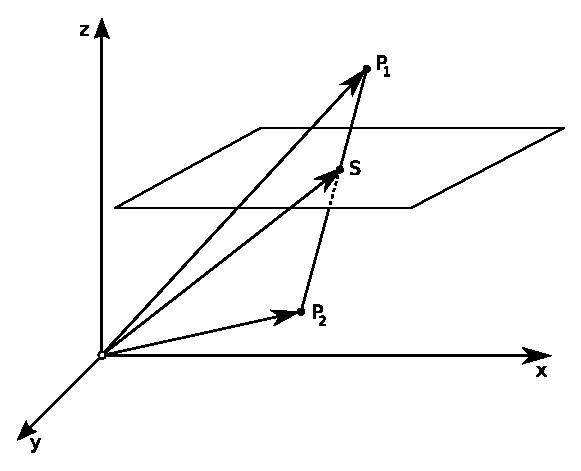
\includegraphics[width=200px]{pictures/sp_gerade_ebene.eps}
    \caption{Schnittpunkt von einer Geraden mit einer Ebene}
    \label{fig:sp_gerade_ebene}
\end{figure}
Exemplarisch soll sich hier auf eine Seite und deren Schnittpunkt mit einer
Ebene beschr"ankt werden.
Gegeben sind die Punkte $P_1$ und $P_2$ und gesucht ist
der Schnittpunkt $S$, wobei die \texttt{z}-Koordinate von $S$ bereits
durch die Ebene
bereits gegeben ist. Folglich sind Insbesondere die \texttt{x}- und die
\texttt{y}-Koordinate von $S$ von Interesse.
Die Punkte k"onnen ebenso als Vektoren betrachtet werden,
wie in der Zeichnung angedeutet. Auch die Kante $\overrightarrow{P_2 P_1}$
kann als
Vektor dargestellt werden durch
\begin{equation*}
    \overrightarrow{P_2 P_1} = P_1 - P_2
\end{equation*}
Da der Schnittpunkt offensichtlich auf diesem Vektor liegen muss, kann $S$
zun"achst wie folgt geschrieben werden:
\begin{equation*}
    S = \lambda \overrightarrow{P_2 P_1}
\end{equation*}
Dabei ist $\lambda$ ein Skalierungsfaktor f"ur den gilt
\begin{equation*}
    \lambda = \frac{z^* - z_2}{z_1 - z_2}
\end{equation*}
Der Wert $z^*$ ist die gegebene \texttt{z}-Koordinate der betrachteten Ebene
und $z_1$ bzw. $z_2$ sind die \texttt{z}-Koordinaten der beiden Punkte $P_1$ und
$P_2$.

Des Weiteren muss ber"uchsichtigt werden, dass $S$ im Moment noch von
$P_2$ und nicht vom Ursprung ausgeht. Um die richtigen Koordinaten von $S$
zu erhalten muss zuletzt noch der Vektor $\vec{P_2}$ zu dem Ergebnis
hinzuaddiert werden, sodass sich f"ur die gesuchten \texttt{x}- und
\texttt{y}-Koordinaten des Schnittpunktes folgende Formeln aufstellen lassen:
\begin{align*}
    x_1^* &= \frac{z^* - z_2}{z_1 - z_2} (x_1 - x_2) + x_2 \\
    y_1^* &= \frac{z^* - z_2}{z_1 - z_2} (y_1 - y_2) + y_2
\end{align*}
Analog lassen sich die Koordinaten $x_2^*$ und $y_2^*$ des Schnittpunktes der
zweiten Kante
berechnen. Zum Schluss werden die Koordinaten aller Schnittkanten in einem
\texttt{edges}-Array gespeichert, wobei eine Kante immer aus vier Koordinaten
besteht,
die hintereinander in das Array eingetragen werden.\\
Mit den so berechneten Schnittkanten kann nun der zweidimensionale
Punkt-in-Polygon-Algorithmus angewandt werden.


\subsection{Punkt-in-Polygon-Algorithmus anwenden}

Durch die im vorherigen Abschnitt {\ref{sec:schnittkanten}} bestimmten
Schnittkanten zwischen der Ebene
und den betroffenen Faces kann im Folgenden der in Kapitel \ref{sec:pip_theo}
bereits theoretisch erl"auterte, zweidimensionale Punkt-in-Polygon-Algorithmus
angewandt werden.\\
Die \texttt{punktInPolygon()}-Methode bekommt hierzu die Koordinaten des zu
testenden Voxels und ein Array mir allen Polygonkanten der Ebene "ubergeben.

\inputminted[linenos=true]{java}{code/PunktInPolygon.java}
Dabei muss f"ur jede Polygonkante gepr"uft werden, ob sie einen Schnittpunkt
mit dem Test-Strahl hat oder nicht. Da jede Kante aus zwei Punkten bzw.
vier Koordinaten besteht, werden diese zu Beginn aus dem \texttt{edges}-Array
geholt und zwischengespeichert.
Schlie\ss lich gibt es nur zwei relevante Zust"ande
(innerhalb und au\ss erhalb),
die in einer Variable \texttt{inside} vom Typ \texttt{boolean} gespeichert
werden k"onnen.\\
Zur effizienteren Berechnung wird der Test-Strahl in Richtung der positiven
\texttt{x}-Achse geschossen.
Um nur die relevanten Kanten auf einen Schnittpunkt mit dem Strahl zu testen,
wird vorab gepr"uft, ob Anfangs- und Endpunkt der aktuellen Polygonkante beide
oberhalb oder beide unterhalb des Teststrahls liegen. Ist dies der Fall, so
kann kein Schnittpunkt vorliegen. Dabei wird die Annahme, dass ein Polygonvertex
infinitesimal "uber dem Test-Strahl liegt, in Zeile 11 und 12 umgesetzt.
Einen Schnittpunkt kann es nur geben, wenn ein Punkt oberhalb und der andere
unterhalb des Strahls liegt, wobei dann die \texttt{x}-Koordinaten genauer
untersucht werden. Liegen beide Punkte rechts von dem zu pr"ufenden Punkt
(d.h. $x1>x$ und $x2>x$), so
schneidet die Kante den Strahl irgendwo und \texttt{inside} wechselt den Wert.
Sind die \texttt{x}-Koordinaten der beiden Punkte kleiner als \texttt{x}, dann
gibt es keinen Schnittpunkt. Liegt ein Punkt rechts und der andere links von
\texttt{x}, so muss berechnet werden, ob der Schnittpunkt rechts von dem
Testvoxel liegt. Ist dies der Fall, so wechselt \texttt{inside} erneut seinen
Wert \cite[S. 51ff.]{skript_cg}.
\\
Das Ergebnis des Punkt-in-Polygon-Algorithmus l"asst sich in Abbildung
\ref{fig:voxel_in_object} gut erkennen. Das erste Bild zeigt die mit Voxeln
gef"ullte Szene und im zweiten Bild sieht man alle Voxel, die innerhalb der
Schachfigur liegen.

\begin{figure}[htbp]
    \centering
    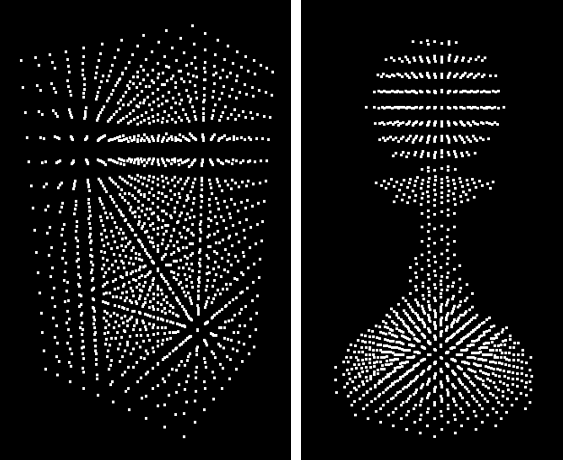
\includegraphics[width=250px]{pictures/voxel_in_object.png}
    \caption{Voxel-in-Objekt-Algorithmus}
    \label{fig:voxel_in_object}
\end{figure}



\section{Marching-Cubes-Algorithmus}
\label{sec:mc_algo}

Der folgende Abschnitt beschreibt die Umsetzung des in Kapitel \ref{sec:mc_theo}
dargestellten Marching Cubes Algorithmus in Java, basierend auf einer
Implementation von Cory Gene Bloyd in C++ \cite{mc_algo}.\\
Um  sp"ater zu bestimmen, an welchen Stellen der Szene Schnee fallen kann, dient
dieser Algorithmus zun"achst als Grundlage, um die Oberfl"ache der Szene bzw.
der Objekte innerhalb der Szene nachzubilden.\\
Gegeben ist das aus Kapitel \ref{sec:voxel_fill} bekannte, regelm"a\ss ige,
dreidimensionale Voxelgitter. Jeder Voxel enth"alt die Information, ob er
innerhalb oder au\ss erhalb eines Objektes liegt.
Es wird nun eine neue Oberfl"ache erstellt, indem man kubusweise durch das
Voxelgrid durchgeht, den jeweiligen W"urfel auf Schnittpunkte mit der
Objektoberfl"ache untersucht und die entsprechenden Dreiecke zeichnet.
Dabei k"onnen verschiedene F"alle auftreten. Die Objektoberfl"ache durchtrennt
den Kubus nicht, sie schneidet einen Vertex ab oder teilt ihn beliebig komplex
in Innen- und Au\ss enbereiche auf. Die Aufteilung richtet sich nach der Anzahl
und dem Index der innen- bzw. au\ss enliegenden Eckvoxeln des Kubus'.
Insgesamt kann es 256 verschiedene F"alle geben, welche bereits in Abbildung
\ref{fig:mc_possibilities} illustriert wurden.\\
Die Bestimmung der Eckpunkte der zu zeichnenden Dreiecke richtet sich nach
der Anzahl und dem Index der geschnittenen W"urfelkanten. Liegt zum Beispiel
ein Voxel innerhalb eines Objekts und ein benachbarter Voxel au\ss erhalb, so
muss die Objektoberfl"ache einen Schnittpunkt mit der Kante zwischen diesen
beiden Voxeln haben. Die genaue Position des Schnittpunktes kann linear
interpoliert werden, worauf in diesem Fall allerdings nicht eingegangen wird.
Stattdessen wird stets der Kantenmittelpunkt als Schnittpunkt gew"ahlt.
%TODO in alle Richtungen interpolieren, nicht nur in z-Richtung!!
%Anschlie\ss end wird in der \texttt{TriangleLookupTable} (TLT) nachgesehen,


\subsection{Imagin"aren Cube erstellen}
Der Marching-Cubes-Algorithmus geht jeden Voxel der Szene durch und bildet
mit diesem Referenzvoxel
einen imagin"aren W"urfel.
Das bedeutet, dass die restlichen sieben Eckvoxel anhand des ersten bestimmt
werden.\\
Die Indizierung der Voxel von \texttt{v0} bis \texttt{v7} sowie die der Kanten
von \texttt{e0} bis \texttt{e11} wie sie bei der Umsetzung des Algorithmus
verwendet werden, ist in Abbildung \ref{fig:cube} dargestellt.

\begin{figure}[htbp]
    \centering
    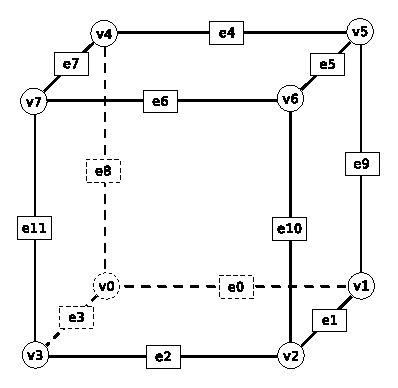
\includegraphics[width=200px]{pictures/cube.eps}
    \caption{Indizierung eines imagin"aren W"urfels}
    \label{fig:cube}
\end{figure}

Der Referenzvoxel ist dabei immer die hintere linke Ecke des Kubus'.
Arbeitet man
mit Vertices, so k"onnen die anderen Eckpunkte mit Hilfe eines Offsets
bestimmt werden. In diesem Fall hingegen werden die Nachbarschaftsbeziehungen
eines Voxels ausgenutzt um dasselbe Ergebnis zu erzielen.

\inputminted[linenos=true]{java}{code/Cube.java}

Wie in dem Codebeispiel zu sehen ist, werden alle acht W"urfelecken in einem
Voxel-Array gespeichert, wobei \texttt{cube[0]} der Referenzvoxel ist.


\subsection{Schnittkanten mit der Ebene bestimmen}

Um im Anschluss die Schnittkanten des W"urfels mit einem Objekt zu ermitteln,
werden alle Eckpunkte darauf getestet, ob sie innerhalb eines Objektes liegen
oder
Schnee beinhalten. Im zweiten Fall wird ein Voxel genauso behandelt wie im
ersten, da er dann bereits in der Schneedecke liegt, folglich unterhalb der
Schneeoberfl"ache.

\inputminted[linenos=true]{java}{code/FlagIntex.java}

Ist der Test erfolgreich, so wird sich dies in einem 8-Bit Index gemerkt
(der \texttt{iFlagIndex}), wobei
jedes Bit einem Eckvoxel entspricht.
Ist ein Voxel innenliegend, so wird das korrespondierende Bit auf 1 gesetzt,
ansonsten bleibt es 0.
Dies geschieht mit einer Bitshift-Operation,die die Zahl \texttt{1} um
die entsprechende Anzahl an Stellen im \texttt{iFlagIndex} nach links
verschiebt.\\
Dieser Teil l"asst sich am Besten anhand eines Beispiels erkl"aren. Es sei
der W"urfel aus Abbildung \ref{fig:cube_example} gegeben. Nun schneidet eine
Objektoberfl"ache
den Kubus derart, dass \texttt{cube[0]} und \texttt{cube[1]} (also \texttt{v0}
und \texttt{v1}) innerhalb des Objektes liegen.
\begin{figure}[htbp]
    \centering
    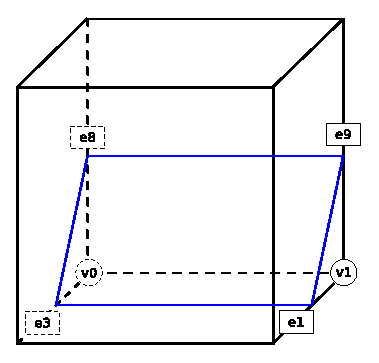
\includegraphics[width=200px]{pictures/cube_example.eps}
    \caption{Beispiel Cube}
    \label{fig:cube_example}
\end{figure}
Der \texttt{iFlagIndex} betr"agt folglich \texttt{0000 0011} in bin"arer oder
\texttt{3} in dezimaler Kodierung.
Als n"achstes wird in einer Tabelle bzw. einem Array nachgesehen, welche
W"urfelkanten von der Oberfl"ache bei gegebenem \texttt{iFlagIndex}
geschnitten werden.

\inputminted[linenos=true]{java}{code/EdgeFlags.java}

Dieses Array hei\ss t \texttt{CubeEdgeFlags}, hat
256 Eintr"age (entsprechend aller Schnittm"oglichkeiten) und bildet den
8-Bit \texttt{iFlagIndex} auf eine 12-Bit kodierte Zahl mit dem Namen
\texttt{iEdgeFlags} ab.

\inputminted[linenos=true]{java}{code/CubeEdgeFlags.java}

Auch hier entpricht jedes Bit einer bestimmten Kante.
Ein Bit ist auf \texttt{1} gesetzt, wenn die Objektoberfl"ache die Kante
schneidet und
\texttt{0}, falls es
keinen Schnittpunkt gibt. Ist \texttt{iEdgeFlags == 0}, so wird keine der
W"urfelkanten geteilt und es
kann mit dem n"achsten Kubus fortgefahren werden.\\
Bezogen auf das obere Beispiel bedeutet dies, dass
\texttt{iEdgeFlags[3] = 0011 0000 1010} in Bin"ar- oder \texttt{0x30a} in
Hexadezimalform beinhaltet.
Das hei\ss t, es werden die Kanten \texttt{e1}, \texttt{e3}, \texttt{e8} und
\texttt{e9} von der Objektoberfl"ache geschnitten, wie auch in Abbildung
\ref{fig:cube_example} zu sehen ist.\\
Anschlie\ss end werden die Koordinaten der Schnittpunkte auf den jeweiligen
Kanten berechnet und in dem zw"olfelementigen \texttt{Vertex}-Array
\texttt{edgeVertex} gespeichert.
Dazu betrachtet man jede Kante und pr"uft, ob in \texttt{iEdgeFlags} an der
entsprechenden Stelle eine \texttt{1} steht. Ist dies der Fall, so folgt
eine Schnittpunktberechnung durch lineare Interpolation.
Bei der Schnittpunktbestimmung wird initial, wie in
Abschnitt \ref{sec:voxel} bereits angek"undigt, der Einfachheit halber von
dem Mittelpunkt einer Kante ausgegangen.
Mit fortschreitendem Anwachsen der Schneedecke richten sich die
auf den W"urfelkanten liegenden Schnittpunkte allerdings nach den
\texttt{density}-Werten der
beiden verbundenen Voxel und werden entsprechend verschoben.\\
Der folgende Codeauschnitt verdeutlicht das oben beschriebene Vorgehen.

\inputminted[linenos=true]{java}{code/Intersection.java}

Die Koordinaten eines Schnittpunktes lassen sich mit Hilfe von drei Hilfsarrays
berechnen. Zun"achst wird im \texttt{EDGE\_CONNECTION}-Array nachgesehen,
welche beiden Voxel die aktuelle Kante verbindet. Danach wird die Entfernung
des Schnittpunktes vom Referenzvoxel durch das
\texttt{VOXEL\_OFFSET}-Array bestimmt. Damit der Vertex an der richtigen Stelle
platziert wird, gibt \texttt{EDGE\_DIRECTION} die Richtung der
Kante an. Der Wert \texttt{0.5f} bedeutet, dass der Kantenmittelpunkt als
Schnittpunkt gew"ahlt wird. \texttt{scale} skaliert schlie\ss lich die
Positionierung in
Abh"angigkeit zur Granularit"at des \texttt{Voxel}-Gitters
($\texttt{scale} = \frac{1}{\texttt{STEPS}}$).\\
Zur besseren Visualisierung werden neben den Schnittpunkten auch
die Einheitsnormalen an eben diesen Punkten berechnet.


\subsection{\texttt{TriangleLookupTable}}

Nachdem alle Schnittpunkte eines Kubus' mit der Objektoberfl"ache berechnet
wurden, m"ussen diese noch in korrekter Reihenfolge zu Dreiecken bzw.
\texttt{Faces} verbunden werden.
Hierzu wird erneut ein Array verwendet, das denselben \texttt{iFlagIndex}
verwendet wie zuvor \texttt{CubeEdgeFlags} und es erlaubt die
\texttt{Vertex}-Sequenz zur Darstellung der angen"ahrten Oberfl"ache
nachzuschlagen. Das \texttt{TriangleLookupTable}-Array ist
zweidimensional und besteht aus \texttt{256 x 16} Eintr"agen, da es
\texttt{256} Teilungsm"oglichkeiten und pro Cube bis zu f"unf \texttt{Faces}
gibt. Die \texttt{TriangleLookupTable} hat die folgende Form.

\inputminted[linenos=true]{java}{code/TriangleLookupTable.java}

Dabei steht die \texttt{-1} f"ur einen invaliden Eintrag und zeigt an, dass
der Algorithmus f"ur diesen Cube an dieser Stelle abgebrochen werden kann
(siehe Zeilen 4-5 im unteren Code-Beispiel).\\

\inputminted[linenos=true]{java}{code/UseTLT.java}

Folglich werden die bis zu f"unf M"oglichkeiten durchgegangen. Soll ein
\texttt{Face} sp"ater gezeichnet werden, so wird auf die
Vertices des \texttt{edgeVertex}-Arrays in richtiger Reihenfolge
zugegriffen und diese werden entgegen dem
Uhrzeigersinn in einer Instanzvariable \texttt{faces} abgespeichert.\\
Erneut bezogen auf den obigen Beispielfall liefert der Aufruf
\texttt{TriangleLookupTable[3]} die Zeile:
\\
\\
\texttt{\{1, 8, 3, 9, 8, 1, -1, -1, -1, -1, -1, -1, -1, -1, -1, -1\}}
\\
\\
Das bedeutet, dass f"ur diesen Cube zwei \texttt{Faces} gezeichnet werden
m"ussen, bestehend aus den Vertices mit den Indizes
\texttt{(1, 8, 3)} und \texttt{(9, 8, 1)}.


\subsection{Ergebnis}
Nachfolgend werden einige Ergebnisse aufgef"uhrt, die mit Hilfe des oben
beschriebenen Algorithmus entstanden sind.
\begin{figure}[htbp]
    \centering
    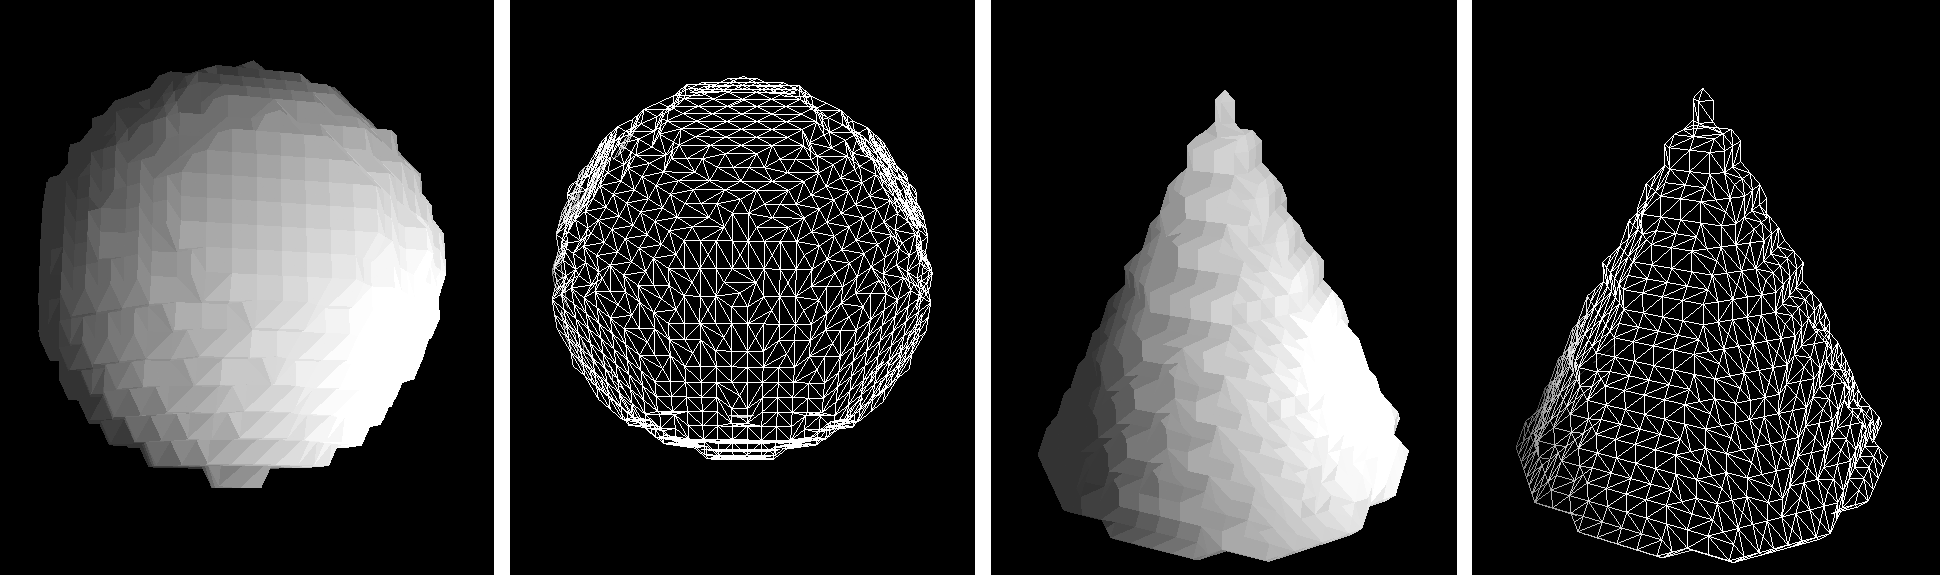
\includegraphics[width=450px]{pictures/mc_objects.png}
    \caption{Marching-Cubes: Ergebnisse}
    \label{fig:mc_result}
\end{figure}
Die Abbildung \ref{fig:mc_result} zeigt im linken Teil die Ann"aherung an
eine Kugel und im rechten die Oberfl"ache eines Kegels.
Damit die erzeugten Dreiecke besser erkennbar sind, ist neben dem jeweiligen
Objekt mit gef"ullten \texttt{Faces} zus"atzlich das entsprechende
Drahtgittermodell dargestellt.\\
Abh"angig von der Voxeldichte kann nun der Detailgrad der erzeugten Oberfl"ache
variiert werden.
Je mehr Voxel vorhanden sind, desto genauer ist die Ann"aherung an die
tats"achliche Objektoberfl"ache. Dies illustriert Abbildung
\ref{fig:granularity} recht deutlich.
\begin{figure}[htbp]
    \centering
    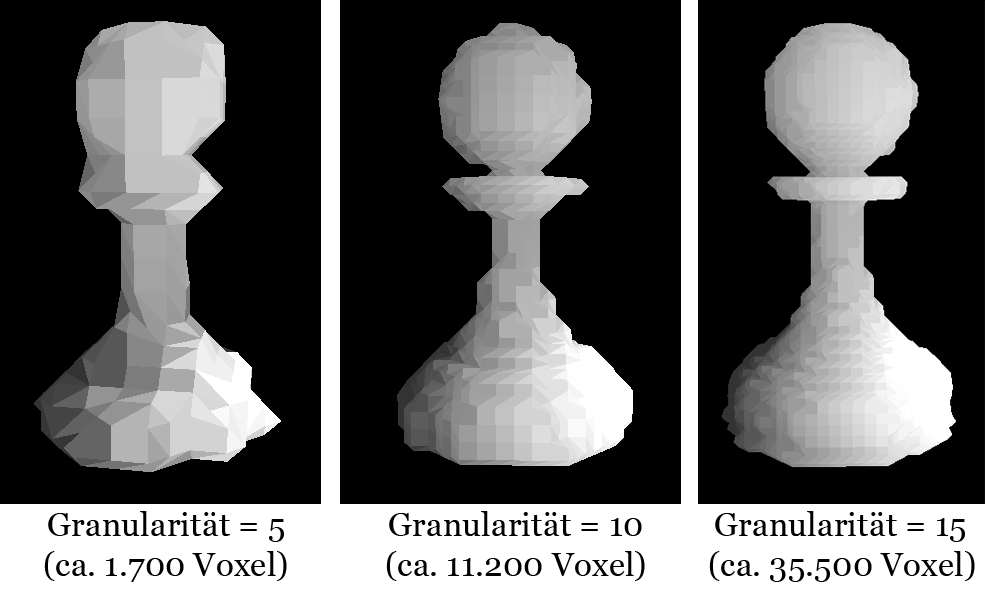
\includegraphics[width=350px]{pictures/granularity.png}
    \caption{Unterschiedlicher Detailgrad des Marching Cubes Algorithmus}
    \label{fig:granularity}
\end{figure}
Allen drei gezeichneten Figuren liegt dasselbe Objekt zugrunde.
Das erste Bild hat offensichtlich eine sehr geringe Voxeldichte von 5
$\frac{Voxel}{Einheit}$. Das hei\ss t pro Einheit auf der jeweiligen Achse
werden 5 Voxel gesetzt. Ist die Szene zum Beispiel 2 Einheiten
(in \texttt{x}-Richtung) lang, so werden 10 Voxel entlang dieser Achse
gesetzt. Das zweite Bild l"asst die Schachfigur deutlich besser erkennen,
da dort 10 Voxel pro Achseneinheit gesetzt werden. Im dritten Bild liegt
schlie\ss lich eine Granularit"at von 15 vor.\\
Nachdem jetzt die Oberfl"ache der Szene durch den Marching-Cubes-Algorithmus
angen"ahert werden kann, ist es im Folgenden m"oglich, Schnee auf Objekte
fallen zu lassen und eine Schneedecke zu erzeugen.


\section{Schneedecke}
\label{sec:snow_surface}
Die zuvor durch den Marching-Cubes-Algorithmus erzeugte Oberfl"ache
dient im Nachfolgenden als Grundlage der Schneedecke. Damit diese allerdings
wachsen und auf den bereits vorhandenen Oberfl"achen aufbauen kann, muss
zun"achst Schneefall simuliert werden. Das Anwachsen der Schneedecke wiederum
wird mit Hilfe der Voxel realisiert, mit denen die gesamte Szene gef"ullt
wurde. Dieses Vorgehen wird im weiteren Verlauf noch genauer erl"autert.\\
Der in diesem Kapitel simulierte Schneefall hat zwei m"ogliche Richtungen:
senkrecht von oben oder schr"ag von der Seite.
Als Abrundung des Ergebnisses wird die
Schneestabilit"at eingef"uhrt. Dabei wird gepr"uft, ob kleinere Lawinen
ausgel"ost werden
m"ussen (Verteilung des Schnees auf benachbarte Voxel), um unrealistisch
hohe Schneeauft"urmungen an Objektkanten zu vermeiden.\\
Die folgenden zwei Applikationsbilder (\ref{fig:mc_initial} und
\ref{fig:rect_obj}) zeigen den initialen Zustand nach einmaliger Anwendung
des Marching-Cubes-Algorithmus'.
\begin{figure}[htbp]
    \centering
    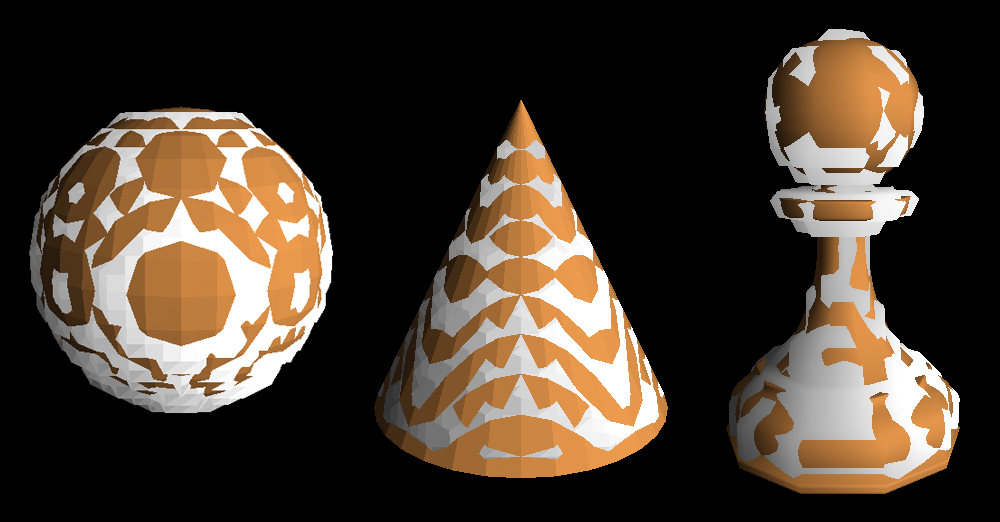
\includegraphics[width=300px]{pictures/mc_initial.png}
    \caption{Unterschied zwischen tats"achlicher und angen"aherter Oberfl"ache}
    \label{fig:mc_initial}
\end{figure}
Die Abbildung \ref{fig:mc_initial} verdeutlicht das in Abschnitt
\ref{sec:voxel} angesprochene Problem der unpr"azisen Ann"aherung an die
tats"achliche Objektoberfl"ache. Die nachgebildete Oberfl"ache,
die als Grundlage der Schneedecke dienen wird, liegt zu Beginn teilweise
"uber und teilweise unter der Oberfl"ache des Objekts.
Ein besseres Ergebnis kann die vorliegende Implementation des Algorithmus'
nicht leisten. Die Gr"unde hierf"ur sind zum einen die Unausgewogenheit
zwischen dem Aufwand der komplexen Berechnung der Schnittpunkte
und dem im
Gegensatz dazu nur leicht verbesserten Endergebnis und zum anderen die
Tatsache, dass die Schneedecke bereits nach wenigen Iterationen auf und "uber
der Objektoberfl"ache liegt, wodurch die zu Anfang durchscheinende Schneedecke
keine Relevanz mehr hat.\\
Im Gegensatz dazu ist die Ann"aherung an rechteckige Objekte, wie in
Abbildung \ref{fig:rect_obj} zu sehen, sehr zufriedenstellend.
\begin{figure}[htbp]
    \centering
    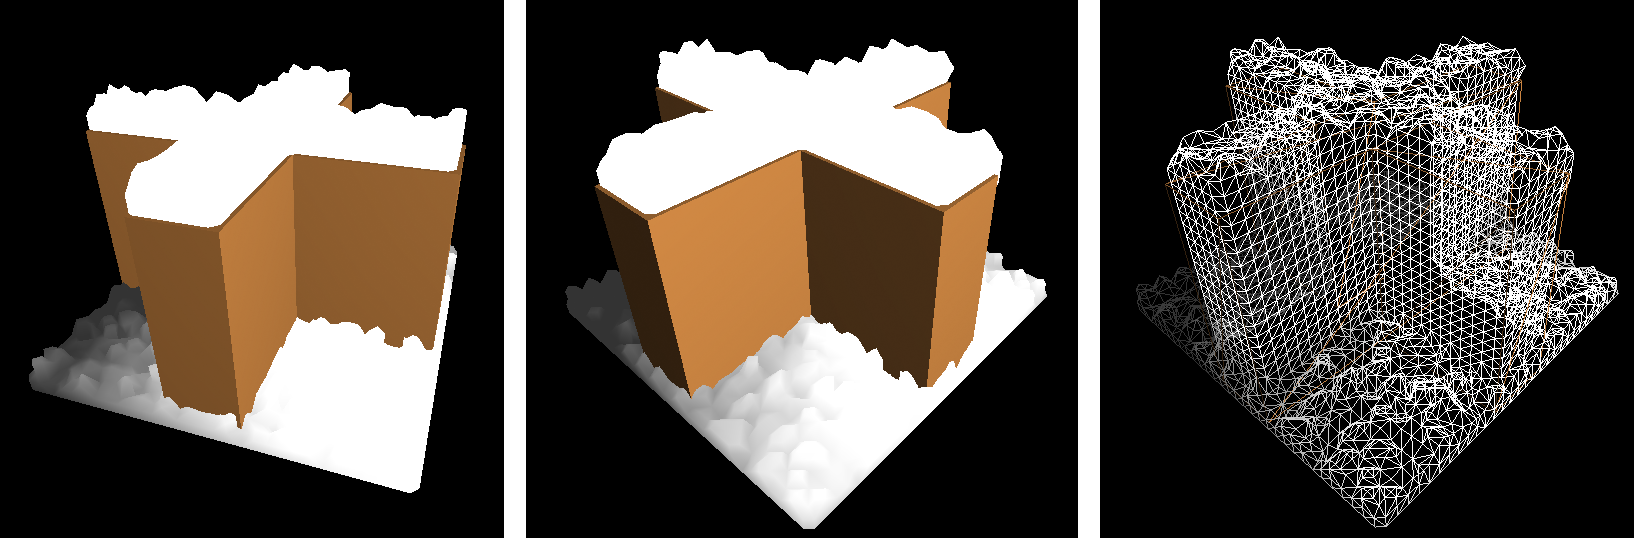
\includegraphics[width=450px]{pictures/rect_obj.png}
    \caption{Ann"aherung eines rechteckigen Objekts mit Schneedecke}
    \label{fig:rect_obj}
\end{figure}


\subsection{Schnee von oben}
Das Anwachsen der Schneedecke soll zun"achst an einem Beispiel verdeutlich
werden. Dabei wird davon ausgegangen, dass die imagin"aren Schneeflocken
senkrecht von oben fallen.
\begin{figure}[htbp]
    \centering
    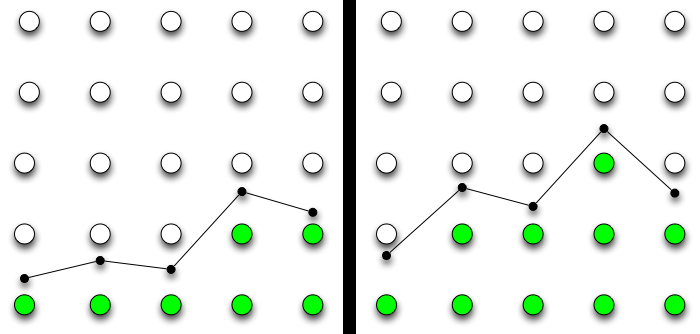
\includegraphics[width=300px]{pictures/voxel_grid_snow.png}
    \caption{Anwachsen der Schneedecke}
    \label{fig:voxel_grid_snow}
\end{figure}
Abbildung \ref{fig:voxel_grid_snow} stellt das Voxelgitter schematisch
und zweidimensional dar. Es werden zus"atzlich die in Abschnitt \ref{sec:voxel}
beschriebenen Eigenschaften der Voxel ausgenutzt.
Die gr"un gef"ullten Kreise repr"asentieren schneegef"ullte Voxel, die kleinen
schwarzen Kreise stellen den jeweiligen \texttt{density}- oder F"ullwert
des darunterliegenden Voxels dar und die schwarze Linie illustriert
die Schneedecke.\\
Der \texttt{density}-Wert eines Voxels kann zwischen \texttt{0} und \texttt{1}
liegen. Er wird erh"oht, wenn eine imagin"are Schneeflocke auf
den jeweiligen Voxel trifft. "Uberschreitet der F"ullwert den Wert
\texttt{1}, so wird mit Hilfe der Nachbarschaftsbeziehung der dar"uberliegende
Voxel aktiviert, das hei\ss t sein \texttt{snow}-Attribut wird auf
\texttt{true}
gesetzt.
Um schlie\ss lich sprunghafte "Uberg"ange von einem Voxel zum n"achsten bei
der Visualisierung des Schneewachstums zu verhindern, wird die
H"ohe der Schneedecke anhand des \texttt{density}-Wertes des entsprechenden
Voxels interpoliert.\\
Im weiteren Verlauf wird nun genauer auf die Umsetzung des senkrechten
Scheefalls auf Programmebene eingegangen. Zur Simulation von Schneefall
oder Schneeflocken m"ussen als erstes die Voxel der Szene bestimmt werden,
auf die Schnee fallen kann. Dazu wird das gesamte
\texttt{Voxel}-Array durchgegangen um anschlie\ss end die in Frage kommenden
Kandidaten im Array \texttt{activeVoxels} zu speichern.
\inputminted[linenos=true]{java}{code/ActiveVoxels.java}
Wird angenommen, dass der Schnee direkt von oben f"allt, so legt das l"angliche
\texttt{if}-Statement (Zeilen 6 - 11) fest, welche Voxel als m"ogliche
Landepl"atze bereitgestellt werden. Dies betrifft zum einen alle auf der
Schneeoberfl"ache liegenden Voxel, also Voxel, die selbst Schnee
enthalten, ihr oberer Nachbar aber nicht. Zum anderen soll auch neben den
Objekten, auf den Szenenboden Schnee fallen k"onnen, wozu die Voxel ohne
unteren Nachbarn aktiviert werden. Zuletzt werden noch die Voxel in Betracht
gezogen, die auf einem Objekt liegen, das hei\ss t der Voxel selbst liegt
innerhalb, sein oberer Nachbar hingegen au\ss erhalb eines Objekts.\\
Sind die aktiven Voxel bestimmt worden, so kann mit der Simulation des
Schneefalls begonnen werden. Dazu bestimmt man zun"achst die Anzahl der
Schneeflocken, die fallen sollen, bevor die Szene neu gezeichnet wird
(in diesem Fall \texttt{int snowflakes = 50}).
\inputminted[linenos=true]{java}{code/TopSnow.java}
Anschlie\ss end wird f"ur jede Schneeflocke ein beliebiger Voxel aus dem
\texttt{activeVoxels}-Array herausgegriffen und dessen \texttt{density}-Wert
um eine konstante Gr"o\ss e erh"oht (z.B. \texttt{0.1}).
"Ubersteigt die \texttt{density} den Wert \texttt{1.0}, so wird der obere
Nachbar des aktuellen Voxels aktiviert und an die Stelle des alten
in das \texttt{activeVoxels}-Array geschrieben.\\
Nach einer gewissen Anzahl von Iterationen f"uhrt dieses Vorgehen zu
dem in Abb. \ref{fig:topSnow} sichtbaren Ergebnis. Der Pfeil zeigt die Richtung
des Schneefalls an.
\begin{figure}[htbp]
    \centering
    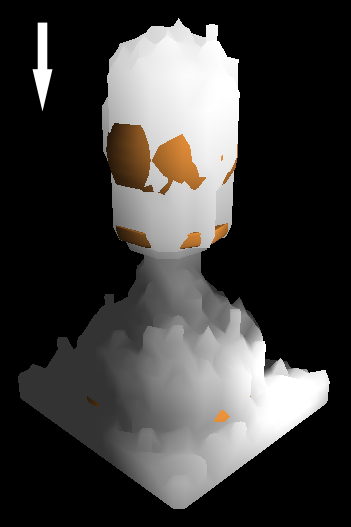
\includegraphics[width=120px]{pictures/topSnow.png}
    \caption{Schneedecke bei senkrechtem Schneefall}
    \label{fig:topSnow}
\end{figure}
Nat"urlich ist dies nur ein grobes Modell zur Validierung und Visualisierung
eines Ergebnisses. Bei dem oben beschriebenen Vorgehen kann es zum Beispiel
vorkommen, dass auch Voxel unterhalb eines Objekts empf"anglich
f"ur Schnee sind, obwohl diese in der Realit"at nicht erreichbar w"aren.
Um ein authentischeres Ergebnis zu erhalten, m"usste ein realit"atsnahes
Partikelsystem erstellt werden, anhand dessen sich Schneeflocken in der Szene
bewegen. In diesem Fall m"usste der \texttt{density}-Wert eines aktiven Voxels
nur erh"oht werden, wenn eine Schneeflocke in das Einzugsgebiet dieses Voxels
f"allt und nicht nach dem oben verwendeten Zufallsprinzip.

\subsection{Schnee von der Seite}
Um Wind zu simulieren wird zus"atzlich zu dem senkrechten noch
waagerechter Schneefall hinzugef"ugt. Die Funktionsweise ist analog zum
Schnee von oben, mit der "Anderung, dass andere Voxel aktiviert werden.
Beispielhaft soll der Schnee von rechts auf das Objekt auftreffen.
\inputminted[linenos=true]{java}{code/RightSnow.java}
Dazu wird lediglich gepr"uft, ob sich ein Voxel auf der Objektoberfl"ache oder
der Schneedecke befindet und einen nicht gef"ullten, rechten Nachbarn besitzt.
Ist dies der Fall, so kann die Schneedecke rechts an das Objekt wachsen.
In Kombination mit den senkrecht fallenden Schneeflocken kann somit ein
Schneefall von rechts oben nachgestellt werden.
Damit das in Abbildung \ref{fig:topRightSnow} dargestellte Ergebnis realistisch
wirkt, ist darauf zu achten, dass die Anzahl der Schneeflocken, die von
oben fallen, gr"o\ss er ist, als die Zahl der von rechts kommenden.
\begin{figure}[htbp]
    \centering
    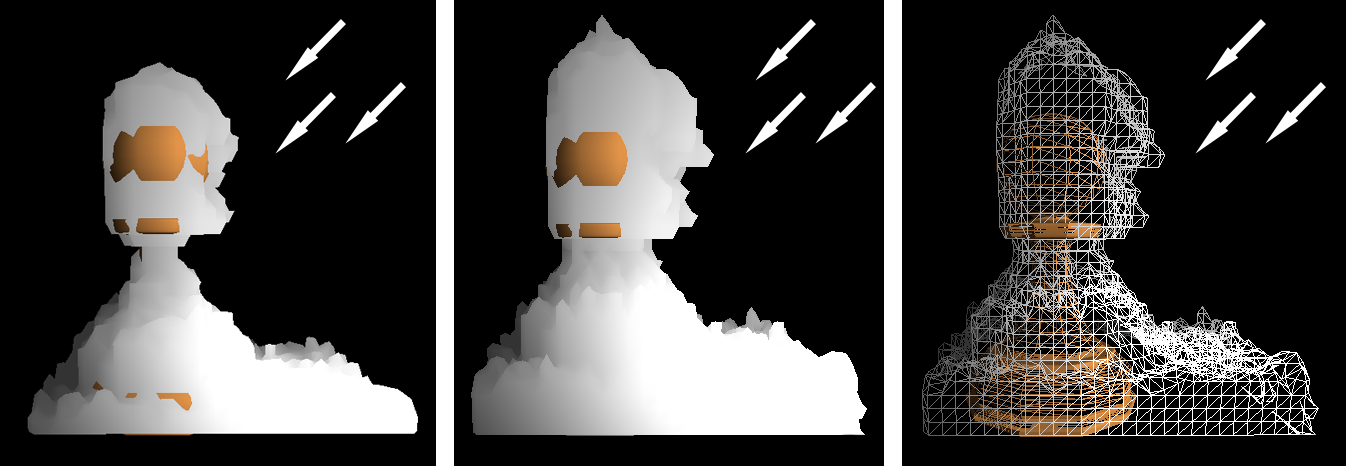
\includegraphics[width=450px]{pictures/topRightSnow.png}
    \caption{Schneedecke bei Schneefall von rechts oben}
    \label{fig:topRightSnow}
\end{figure}
Zudem zeigen die ersten beiden Bilder zwei Zust"ande der Szene mit steigender
Schneedecke. Im dritten Bild verdeutlicht das Drahtgittermodell gut die
deutlich nach oben und nach rechts gewachsene Schneedecke, da sich die
Schachfigur darunter erkennen l"asst.


\subsection{Schneestabilit"at}
Die Idee des Stabilit"atstests der Schneedecke stammt aus dem Paper
\glqq Computer Modelling Of Fallen Snow\grqq\ von Paul Fearing, in dem
er sich ebenfalls mit der Akkumulation von Schnee sowie der Bildung von
Schneedecken besch"aftigt, dabei allerdings einen anderen Ansatz verfolgt
\cite{fallen_snow}.\\
Die Notwendigkeit eines solchen Tests wird deutlich, wenn man sich das bisher
erzeugte Ergebnis einer Schneepunktquelle ansieht. Es entsteht lediglich eine
grotesk wirkende, steile und sehr schmale S"aule. In der Realit"at hingegen
erwartet man, dass aufgrund der geringer werdenden Stabilit"at Lawinen
ausgel"ost werden, wenn auch nur in sehr kleinem Ma\ss stab, und sich der
Schnee von
dem obersten Punkt auf den Boden um diesen herum verteilt. Somit sollte
nach einer gewissen Zeit ein kegelf"ormiger Schneehaufen entstehen.
Die Vor"uberlegungen sowie der schematische Ablauf des Stabilit"atstest und
der Umverteilung der Schneemenge werden in Abbildung \ref{fig:stability}
verdeutlicht.
\begin{figure}[htbp]
    \centering
    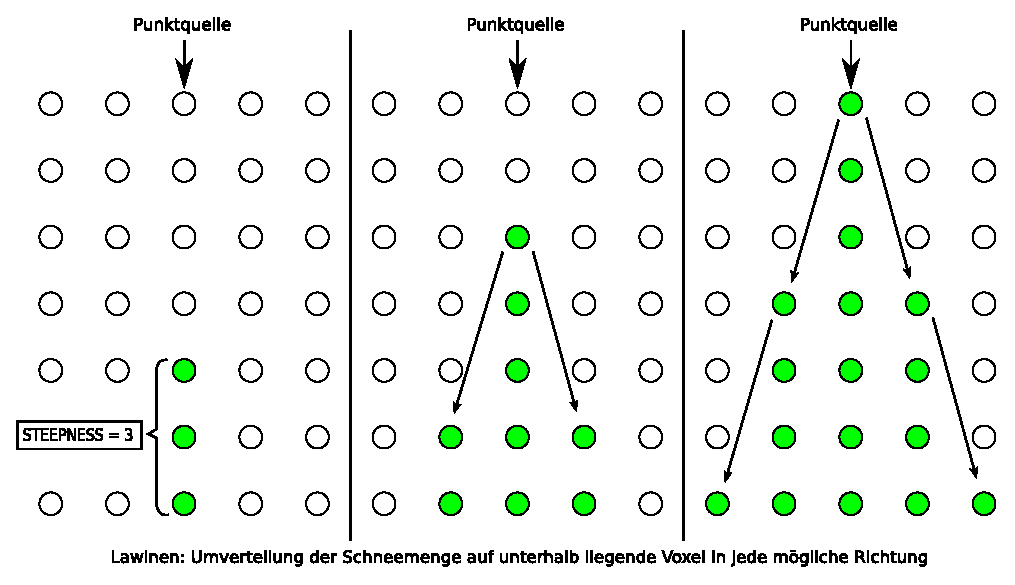
\includegraphics[width=400px]{pictures/stability.eps}
    \caption{Darstellung des Lawinenprinzips}
    \label{fig:stability}
\end{figure}
Gegeben sei eine Punktquelle, von der aus der Schnee gerade nach unten f"allt.
Eine Lawine wird dann ausgel"ost, falls der H"ohenunterschied zwischen einem
schneebeinhaltenden Voxel und einem seiner Nachbarn zu gro\ss\ geworden ist.
Der maximal erlaubte H"ohenunterschied wird durch die Konstante
\texttt{STEEPNESS}, also die gew"unschte Steilheit der Schneedecke festgelegt.
In den hier aufgef"uhrten Beispielen wird mit einer \texttt{STEEPNESS}
von \texttt{3} gearbeitet, da dieser Wert zufriedenstellende Ergebnisse erzeugt.
Die Bilder 2 und 3 der Abbildung \ref{fig:stability} stellen den weiteren
Verlauf und die Ver"anderung der Schneedecke bei gleichbleibendem, punktuellem
Schneefall dar.\\
Der im Folgenden anhand von Code-Beispielen erk"arte Algorithmus zur
Stabilit"atspr"ufung wird immer dann ausgef"uhrt,
wenn der \texttt{density}-Wert eines Voxels erh"oht wurde.
\inputminted[linenos=true]{java}{code/StabilityTest.java}
Die Methode \texttt{stabilityTest()} bekommt einen \texttt{Voxel} "ubergeben
und pr"uft f"ur jeden Nachbarn, ob er Schnee an diesen abgeben muss.
Dieser Fall tritt ein, wenn der aktuelle Voxel mehr als die erlaubte
H"ohendifferenz (\texttt{STEEPNESS}) zu seinem Nachbarn aufweist.\\
Ermittelt wird diese mit Hilfe der \texttt{height()}-Methode. \texttt{height()}
bekommt ebenfalls einen \texttt{Voxel} "ubergeben und z"ahlt in einer
\texttt{while}-Schleife die Anzahl der \texttt{Voxel}, die nach unten
gegangen werden kann, bevor man auf den Boden, eine Schneeoberfl"ache oder
ein Objekt trifft.
\inputminted[linenos=true]{java}{code/Height.java}
Da der Code des Stabilit"atstest f"ur alle Nachbarn analog funktioniert, wurde
beispielhaft die Pr"ufung des rechten Nachbarvoxels herausgegriffen.\\
"Ubersteigt die ermittelte H"ohendifferenz nun den zul"assigen Wert, so
muss eine Umverteilung der Schneemenge vorgenommen werden. Dazu ermittelt
die Methode \texttt{avalanche()} zun"achst den Voxel, auf den die Lawine
treffen soll. Dies geschieht nach demselben Prinzip wie in der
\texttt{height()}-Methode, mit dem Unteschied, dass
ein \texttt{Voxel} und kein \texttt{int} zur"uckgeliefert wird.\\
Wurde der entsprechende Voxel bestimmt, so wird sein \texttt{density}-Wert
um einen Bruchteil der Schneeflocke erh"oht, die auf den h"ohergelegenen
Nachbarn gefallen ist. Damit eine ansehnliche Kegelform entstehen kann hat
sich gezeigt, dass die folgende Verteilung gute Ergebnisse liefert. Die
\texttt{density} der
in der Von-Neumann-Nachbarschaft liegenden Voxel (vorne, hinten, links, rechts)
erh"oht sich jeweils um $\frac{1}{6}$ des Schneeflockenwertes und die restlichen
(hinten links, hinten rechts, vorne links, vorne rechts)
bekommen jeweils $\frac{1}{12}$ der Schneeflocke ab. Diese Untescheidung ist
wichtig, denn bei gleichm"a\ss iger Aufteilung w"urde sich kein kegel- sondern
stattdessen ein pyramidenf"ormiger Schneeberg bilden.\\
Da sich nach der ersten Umverteilung bereits neue, invalide H"ohendifferenzen
gebildet haben k"onnen, wird der Stabilit"atstest rekursiv mit dem zuvor
aktualisierten Nachbarn aufgerufen.\\

In Abbildung \ref{fig:singleTopSnow} ist schlie\ss lich das Ergebnis des
Stabilit"atstests an einem Beispiel zu sehen. Die Szene beihnaltet dabei
eine im Raum schwebende
Kugel auf die mittig von oben aus einer Punktquelle Schnee f"allt.
\begin{figure}[htbp]
    \centering
    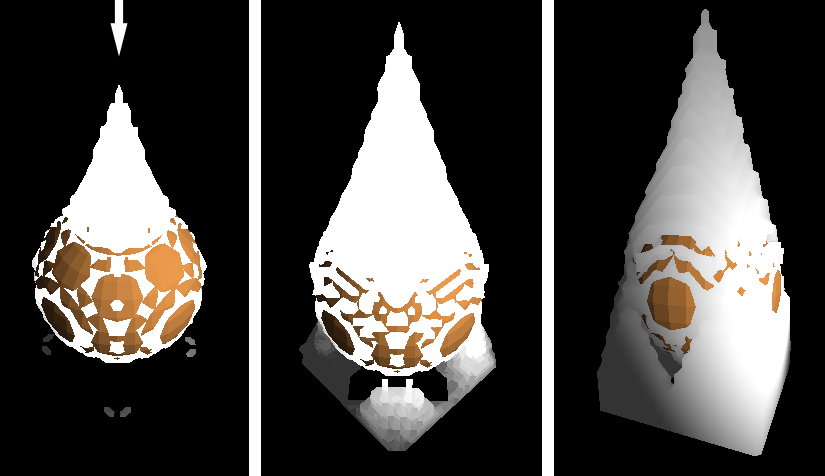
\includegraphics[width=300px]{pictures/singleTopSnow.png}
    \caption{Schneeverteilung bei einer Punktquelle mit Stabilit"atstest}
    \label{fig:singleTopSnow}
\end{figure}
Der sich bildende Schneekegel auf der Kugel ist deutlich sichtbar.
Zudem kann man erkennen, dass der Schnee an den Seiten der Kugel herunterf"allt,
sobald kein Platz mehr auf der Oberfl"ache vorhanden ist. Die Simulation
verh"alt sich folglich wie gew"unscht und erzeugt ein gutes Ergebnis.\\

%\begin{figure}[htbp]
%    \centering
%    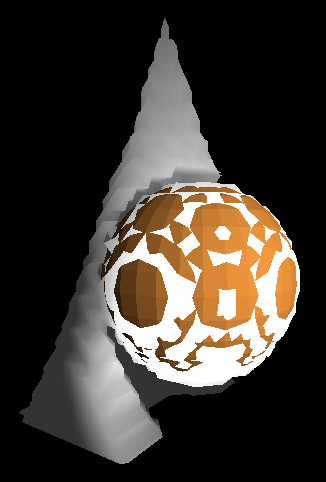
\includegraphics[width=120px]{pictures/singleTopSnow_versetzt.png}
%    \caption{Beispiel der Schneeverteilung bei alternativer Punktquelle}
%    \label{fig:singleTopSnow_versetzt}
%\end{figure}
In einem letzten Schritt soll schlie\ss lich der randomisierte, senkrechte
Schneefall mit dem Stabilit"atstest kombiniert werden.
Das Endergebnis dieser Kombination zeigt die Abbildung
\ref{fig:topSnowStability} in einem Vorher-Nachher-Vergleich.
\begin{figure}[htbp]
    \centering
    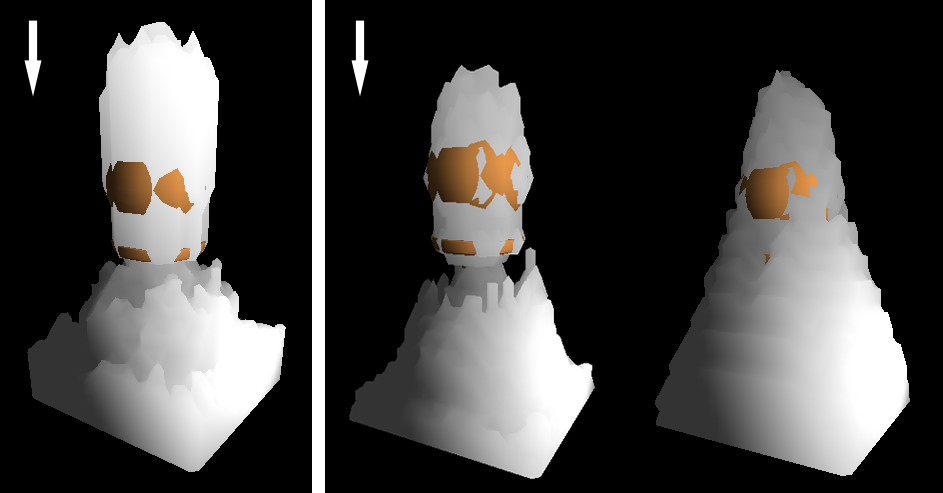
\includegraphics[width=300px]{pictures/topSnowStability.png}
    \caption{Senkrechter Schneefall ohne und mit Stabilit"atstest}
    \label{fig:topSnowStability}
\end{figure}
Im linken Bild ist der Schneefall ohne Stabilit"atstest zu sehen. Sehr
auff"allig sind hier die unrealistisch hohen Schneekanten auf dem Kopf der
Schachfigur. Unter der Anwendung des Stabilit"atstests dagegen werden wesentlich
bessere Ergebnisse geliefert (rechtes Bild). Dabei kann sich nur eine bestimmte
Menge Schnee auf dem Bauernkopf sammeln, bevor diese, wie auch in dem vorherigen
Beispiel, in kleineren Lawinen auf die darunterliegenden Nachbarvoxel verteilt.


%%%%%%% REFLEXION %%%%%%%%

\chapter{Reflexion}
In diesem Kapitel werden zun"achst die Ergebnisse der Arbeit kurz
zusammengefasst und deren G"ute diskutiert. Abschlie\ss end folgt ein Fazit und
ein Ausblick auf m"ogliche Optimierungen des vorgestellten Verfahrens.

\section{Zusammenfassung}
Die im Zuge dieser Arbeit entstandene Applikation erf"ullt das zu Anfang
aufgestellte Ziel der Generierung einer Schneedecke in vollem Umfang.
Es wird mit Hilfe prozeduraler Techniken eine Schneedecke f"ur eine beliebige
Szene modelliert. Dabei ist lediglich zu beachten, dass die erstellte
Szene in dem beschriebenen Wavefront-Format vorliegt, damit das
Programm in der Lage ist, diese zu analysieren und auszulesen.\\
Nachdem verschiedene L"osungsans"atze diskutiert wurden, fiel die Wahl auf
eine Umsetzung der Schneerepr"asentation durch sog. Voxel, da dieses
Verfahren vielversprechende Ergebnisse erhoffen lie\ss.
Das Vorgehen und der Ablauf des Programms sind in der Snow-Pipeline
(Abbildung \ref{fig:snow_pipeline}, Kapitel \ref{sec:voxel}) pr"agnant
zusammengefasst.\\
%TODO evtl. mehr zur zusammenfassung schreiben


\section{Fazit und Ausblick}
Im Rahmen dieser Arbeit war es leider nicht m"oglich, noch andere Verfahren zur
Schneedeckengenerierung umzusetzen um diese dann gegebenenfalls in Bezug auf
Effizienz und Qualit"at mit der vorliegenden Realisierung zu vergleichen.
Zudem konnten aufgrund der beschr"ankten Zeit und der teilweise hohen
Komplexit"at einige Funktionalit"aten nicht implementiert
werden, die zu weiteren Ergebnisverbesserungen gef"uhrt h"atten. Somit ist
das Potential des Verfahrens noch nicht vollst"andig ausgereizt.
Zum Beispiel ist der 
simulierte Schneefall lediglich durch einen randomisierten Arrayzugriff
realisiert. Dabei f"allt der Schnee auf zuvor ermittelte
aktive Voxel, die sich momentan noch unter einem Objektvorsprung
befinden k"onnen. Dies hat zur Folge, dass sich auch an Stellen Schnee
sammeln kann, wo in der Realit"at kein Schnee fallen w"urde. 
Abhilfe k"onnte hier ein Partikelsystem schaffen, welches Schneeflocken
realit"atsnah durch den Raum bewegt. Dabei k"onnten der Wind, die
Gravitation und
im Weg befindliche Objekte die Bewegungsrichtung einer solchen Flocke bestimmen,
bevor diese auf den Boden bzw. die Schneedecke trifft, an dessen Stelle
schlie\ss lich der \texttt{density}-Wert des entsprechenden Voxels erh"oht
w"urde. Damit lie\ss en sich ebenfalls Schneeverwehungen oder -verwirbelungen
darstellen.\\
Eine weitere Verbesserungsm"oglichkeit ist bei der initialen Ausf"uhrung des
Marching-Cubes-Algorithmus' gegeben. Wie in Abschnitt \ref{sec:voxel} bereits
erl"autert und in
Abbildung \ref{fig:mc_initial} illustriert, liefert die erste Iteration des
Algorithmus lediglich eine grobe Ann"aherung an die in der Szene vorhandenen
Objekte, was besonders bei nicht-rechteckigen Objekten ins Auge f"allt.
Dieses Problem verliert zwar an Relevanz je mehr Schnee gefallen ist
und desto h"oher die Schneedecke anw"achst, jedoch lie\ss e sich das Ergebnis
durch eine genaue Schnittpunktberechnung der W"urfelkanten mit der
Objektoberfl"ache weiter verbessern.
Ein abschlie\ss end erw"ahnenswerter Makel ist der lediglich geringe
Detailgrad einer m"oglichen Schneeoberfl"ache. Damit ist gemeint, dass
nur eine recht grobe Bedeckung der Szene erreicht werden kann. Das stellt kein
Problem bei gro\ss en Objekten wie Erhebungen in der Landschaft oder Geb"auden
dar. Kleinere Details
hingegen, wie zum Beispiel die "Aste eines Baums werden h"ochstwahrscheinlich
nicht von dem Algorithmus erfasst, da das Voxelgitter zu grob ist.
Nun einfach die Voxeldichte zu erh"ohen, ist keine realistische Option, da man
diese wirklich sehr hoch ansetzen m"usste um auch kleinere Details mit
Schnee zu bedecken, was wiederum die Anzahl der Voxel zu einer unpraktikabel
gro\ss en Menge anwachsen lie\ss e, die schlie\ss lich nicht mehr effizient
zu verwalten w"are.\\
Folglich k"onnte man sich durchaus weitere Arbeiten in dem Bereich vorstellen,
die entweder auf dieser Arbeit aufbauen oder einen komplett anderen Ansatz
verfolgen und diesen dann mit dem hier umgesetzten vergleichen.\\
%TODO evtl, noch was zur Projektgruppe schreiben

Zusammenfassend l"asst sich sagen, dass die Repr"asentation einer Schneedecke
durch ein Voxelgrid 
%TODO vllt. noch etwas zu MC und Stabilit"at sagen...
ein durchaus zufriedenstellendes Ergebnis erzeugt, auch wenn dieses
eventuell noch verbesserungsf"ahig ist.

% DON'T set \bibliographystyle here -- use the documentclass option instead
\bibliography{papers}

\closing %%%%%%%%%%%%%%%%%%%%%%%%%%%%%%

\end{document}
